\documentclass[9pt,dvipdfmx,a4paper]{jsarticle}

\usepackage{amsmath,amssymb}
\usepackage{bm}
\usepackage[dvipdfmx]{graphicx}
\usepackage{physics} % http://mirrors.ibiblio.org/CTAN/macros/latex/contrib/physics/physics.pdf
\usepackage{siunitx} %SI単位を楽に出力
\usepackage{mathtools} %環境の追加
\usepackage{circuitikz} %電気回路をtex中で書く
% \usepackage{caption} %番号なしキャプションを書く
% \usepackage{cancel} %式中に斜線を入れる
% \usepackage{tensor} %テンソルの添え字を書く
% \usepackage{tikz} %図を書く
% \usepackage{ascmac} %四角い枠の中に文章を書く
% \usepackage{float} %figureで[hbp]オプションを使う
% \usepackage{hyperref}  \usepackage{pxjahyper} %ハイパーリンクをつかう
% \usepackage{tablefootnote} %表中に注釈をいれる
% \usepackage[thicklines]{cancel} %数式中の取り消し線
\usepackage[version=4]{mhchem} %化学式の入力
\usepackage{pdfpages}
\usepackage{wrapfig} %文章の回り込み
\usepackage[subrefformat=parens]{subcaption} %(a)図のようにすることができるやつ
\usepackage{here}
\usepackage{mathrsfs} % フォントの追加
\usepackage{url} % url を入れる
\usepackage[margin=15mm]{geometry} %余白の削除
\usepackage{tcolorbox}
% \usepackage{tikz-feynhand}

\renewcommand{\abstractname}{Abstract}

\usepackage{fancyhdr}
\pagestyle{fancy}
\lhead{応用物理学実験:ファラデー効果}
\rhead{1522068 西原 翔}
\cfoot{\thepage}

\graphicspath{{./image/}}

\begin{document}

%出力したpdfを表紙にするとき
% \includepdf[pages=1,noautoscale=false]{cover.pdf}
% \newpage

%texで表紙を書くとき
\quad\\[35mm]
\centerline{\Huge{\textsf{第 10 回}}}
\quad\\[5mm]
\centerline{\Huge{\textsf{応 用 物 理 学 実 験}}}
\quad\\[5mm]
\begin{table}[h]
	\centering
	\begin{tabular}{| c | c |}
		\hline
		\Huge\textsf{{題目}} & \Huge{\textsf{ファラデー効果}} \rule[-5mm]{0mm}{15mm} \\
		\hline
	\end{tabular}
\end{table}
\quad\\[10mm]
\begin{table}[h]
	\centering
	\begin{tabular}{l l}
		\hline
		\LARGE{\textsf{氏\qquad 名}} & \LARGE{\textsf{: 西原 翔}} \rule[0mm]{0mm}{6mm} \\
		\hline
		\LARGE{\textsf{学  籍  番  号}} & \LARGE{\textsf{: 1522068}} \rule[0mm]{0mm}{6mm} \\
		\LARGE{\textsf{学部学科学年}} & \LARGE{\textsf{: 理学部第一部応用物理学科3年}}\\
		\hline
	\end{tabular}
\end{table}
\quad\\[10mm]
\centerline{\LARGE{\textsf{共同実験者:1522064 中井空弥}}}\\[2mm]
% \centerline{\LARGE{\textsf{\qquad\qquad\quad\;\;1522091 宮田祟杜}}}\\[2mm]
% \centerline{\LARGE{\textsf{\qquad\qquad\quad\;\;1522095 村山涼矢}}}\\[2mm]
% \centerline{\LARGE{\textsf{\qquad\qquad\quad\;\;1522B02 中村洸太}}}\\[2mm]
\quad\\[10mm]
\centerline{\LARGE{\textsf{提出年月日:2024年12月19日}}}\\[2mm]
\centerline{\LARGE{\textsf{実験実施日:2024年11月29日}}}\\[2mm]
\centerline{\LARGE{\textsf{\qquad\qquad\quad\;2024年12月06日}}}
\quad\\[10mm]
\centerline{\LARGE{\textsf{東 京 理 科 大 学 理 学 部 第 1 部}}}\\[2mm]
\centerline{\LARGE{\textsf{応 用 物 理 学 教 室}}}

\thispagestyle{empty}
\clearpage
\addtocounter{page}{-1}
\newpage

% \twocolumn

\begin{abstract}
    This report presents the theoretical and experimental investigation of the Faraday effect,
    which involves the rotation of the polarization plane of light passing through a magnetized medium.
    The principles of light polarization, including Jones vectors and matrices,
    are reviewed to describe changes in polarization states induced by optical elements.
    Experimental setups utilizing He-Ne lasers, polarizers,
    and \(\lambda/4\) plates are detailed for analyzing linearly polarized and circularly polarized light.
    The Faraday effect is explored using magneto-optical glass with applied magnetic fields,
    with results indicating a proportional relationship between the polarization rotation angle
    and the magnetic field strength. Discrepancies between experimental Verdet constants and reference values are discussed,
    with potential sources of error including material properties and measurement inaccuracies.
    Applications of the Faraday effect in optical communication devices, such as isolators, are also addressed.
\end{abstract}


\section{原理}
\subsection{光の偏光とジョーンズベクトル}
光は電磁波であるため、これはマクスウェル方程式に従う。
電荷分布のない媒質中での光はガウスの法則
\begin{align}
    \div{\vb*{E}} = 0 \overset{FT}{\qquad\rightarrow\qquad} \vb*{k}\cdot \vb*{E} = 0
\end{align}
より横波であるのがわかる。
光の進行方向を法線とする平面を自由に振動することから、
2つの独立な成分を持つ。これを偏光という。

2つの偏光の位相差も含めた光電場を表記するのにジョーンズベクトルと呼ばれるものがある。
これは\(z\) 軸に進む光で全体の位相が \(kz-\omega t\) で書けるとき
\footnote{光子数が一定(\(\simeq\)強度が一定)のレーザー光は光子数と位相の不確定性より、このように書けない}、
\(x,\,y\) 平面の電場のベクトルを
\begin{align}
    \vb*{E} = e^{i(kz-\omega t)}
    \begin{pmatrix}
        E_{0x}\\ E_{0y}e^{i\phi}
    \end{pmatrix}
\end{align}
のようにして表すものである。
ベクトルの第 1 成分は \(x\) 軸に関する光電場の振動、つまり横偏光を、
ベクトルの第 2 成分は \(y\) 軸に関する光電場の振動、つまり縦偏光表している。
\(e^{i\phi}\)は横偏光と縦偏光の相対位相を表している項である。

このジョーンズベクトルを用いると様々な偏光状態を表すことができる。
このベクトルの実部を取ると
\((E_x,\,E_y) = (E_0\cos\theta\cos(kz-\omega t),\,E_0\cos\theta\cos(kz-\omega t+\phi) )\)となる。
これから \(kz-\omega t\)の部分を消すように変形すると、
\begin{align}
    \qty(\frac{E_x}{E_{0x}})^2 + \qty(\frac{E_y}{E_{0y}})^2
    - \frac{2\cos\phi E_x E_y}{E_{0x}E_{0y}} = \sin^2\phi
\end{align}
という楕円の式が得られる。
つまり、光電場ベクトルは一般的には楕円の周上を回転しながら進んでいくとわかる。
これを楕円偏光という。

光電場の横成分と縦成分の位相差がない(\(\phi=0\))とき、もしくは逆位相のとき(\(\phi=0\))、
この場合には(3)式から
\begin{align}
    \frac{E_x}{E_{0x}} = \pm \frac{E_y}{E_{0y}}
\end{align}
が得られる。これは直線状を光電場ベクトルを上を動くので、この光の偏光は直線偏光であるという。

光電場の横成分と縦成分の大きさが同じ (\(E_{0x}=E_{0y}\equiv E_0\)) かつ位相差が\(\phi=\pm\pi/2\)のとき
(3) 式から
\begin{align}
    E_x^2 + E_y^2 = E_0^2
\end{align}
という円の式が得られる。円周上を回る偏光であるので、これを円偏光という。
これに対応するジョーンズベクトルを
\begin{align}
    \vb*{r} = \frac{1}{\sqrt{2}}
    \begin{pmatrix}
        1\\i
    \end{pmatrix},\qquad
    \vb*{l} = \frac{1}{\sqrt{2}}
    \begin{pmatrix}
        1\\-i
    \end{pmatrix}
\end{align}
というようにおく。
前者を光の進行方向に対して右回りに回る偏光であるので右回り円偏光、
後者を光の進行方向に対して左回りに回る偏光であるので左回り円偏光と呼ぶ。
また、このベクトルは正規直交しているので、
これを偏光ベクトルの基底として扱うこともできる。
物質との相互作用を考える際にはこちらが便利であることがある。

\subsection{光学素子とジョーンズ行列}
光が光学素子によってその状態が変わるというのは、ジョーンズベクトルに行列が作用するというように理解できる。
透過した光が x 方向の直線偏光となる偏光板は行列を用いて
\begin{align}
    \hat{P}_x =
    \begin{pmatrix}
        1 & 0\\
        0 & 0
    \end{pmatrix}
\end{align}
というように書くことができる。
このようにおくことで\(\hat{P}_x \vb*{E}\)としたときに、
縦偏光の成分がなくなるのがわかる。
また、この偏光板を角度 \(\theta\) だけ回転させたものは回転行列\(R(\theta)\)を用いて
\begin{align}
    \hat{P}(\theta) = \hat{R}(\theta)\hat{P}_x \hat{R}^{-1}(\theta)
    = \begin{pmatrix}
        \cos \theta & -\sin\theta\\
        \sin\theta & \cos\theta
    \end{pmatrix}
    \begin{pmatrix}
        1 & 0\\
        0 & 0
    \end{pmatrix}
    \begin{pmatrix}
        \cos \theta & \sin\theta\\
        -\sin\theta & \cos\theta
    \end{pmatrix}
    =\begin{pmatrix}
        \cos^2 \theta & \cos\theta\sin\theta\\
        \cos\theta\sin\theta & \sin^2\theta
    \end{pmatrix}
\end{align}
というようにあらわせる。

横偏光と縦偏光の位相を\(\phi\)だけずらす移相子はこのように書ける。
\begin{align}
    \hat{\Delta}_\phi(\theta) &= \hat{R}(\theta) \hat{\Delta}_\phi  \hat{R}^{-1}(\theta) \notag\\
    &= \begin{pmatrix}
        \cos \theta & -\sin\theta\\
        \sin\theta & \cos\theta
    \end{pmatrix}
    \begin{pmatrix}
        1 & 0\\
        0 & e^{i\phi}
    \end{pmatrix}
    \begin{pmatrix}
        \cos \theta & \sin\theta\\
        -\sin\theta & \cos\theta
    \end{pmatrix}
    =e^{i\phi} \hat{I} + (1-e^{i\phi})\begin{pmatrix}
        \cos^2 \theta & \cos\theta\sin\theta\\
        \cos\theta\sin\theta & \sin^2\theta
    \end{pmatrix}.
\end{align}
ここで \(\hat{I}\)は単位行列を表している。

移相子のうち位相を \(\phi = \pi/2\) ずらすものを \(\lambda/4\) 板といい、
\begin{align}
    \hat{Q}(\theta)
    =i\hat{I} + (1-i)\begin{pmatrix}
        \cos^2 \theta & \cos\theta\sin\theta\\
        \cos\theta\sin\theta & \sin^2\theta
    \end{pmatrix}
    =\begin{pmatrix}
        \cos^2\theta+i\sin^2\theta & (1-i)\cos\theta\sin\theta\\
        (1-i)\cos\theta\sin\theta & \sin^2\theta + i \cos^2\theta
    \end{pmatrix}
\end{align}
というように書く。
角度を \(\theta = 0\) として、直線偏光 \(\vb*{d}=\,^t(1,0)/\sqrt{2}\) を \(\lambda/4\) 板に通すと、
\begin{align}
    \hat{Q}(0)\vb*{h} =\frac{1}{\sqrt{2}}
    \begin{pmatrix}
        1   &   0\\
        0   &   i
    \end{pmatrix}
    \begin{pmatrix}
        1 \\ 1
    \end{pmatrix}
    = \frac{1}{\sqrt{2}}\begin{pmatrix}
        1 \\ i
    \end{pmatrix}
    =\vb*{r},
\end{align}
円偏光 \(\vb*{r} = \,^t(1,i)/\sqrt{2}\) を \(\lambda/4\) 板に通すと、
\begin{align}
    \hat{Q}(0)\vb*{r} = \frac{1}{\sqrt{2}}
    \begin{pmatrix}
        1   &   0\\
        0   &   i
    \end{pmatrix}
    \begin{pmatrix}
        1 \\ i
    \end{pmatrix}
    = \frac{1}{\sqrt{2}}\begin{pmatrix}
        1 \\ -1
    \end{pmatrix}
    \equiv\vb*{a},
\end{align}
というようになる。
つまり、\(\lambda/4\) 板は直線偏光を円偏光に、
円偏光を直線偏光に変換する素子であるとわかる。

このような行列ジョーンズベクトルに作用して偏光状態を変える行列はジョーンズ行列と呼ばれる。
始めの光電場が \(\vb*{E}\) でジョーンズ行列 \(\hat{J}\) で表せる光学素子を通ったあと、
実際に測定される光の強度は
\begin{align}
    I = \abs{\hat{J}\vb*{E}}^2
\end{align}
というようになる。

% 一般の楕円偏光 \(^t(\cos\theta,e^{i\phi}\sin{\theta})\) を偏光版\(\hat{P}(0)\)を通すことで得られる光の強度は
% \begin{align}
%     I = \abs{\begin{pmatrix}
%         1   &   0\\
%         0   &   0
%     \end{pmatrix}\begin{pmatrix}
%         \cos\theta \\ e^{i\phi}\sin\theta
%     \end{pmatrix}}^2 = \cos\theta^2
% \end{align}
% というようになる。

% 一般の楕円偏光 \(^t(\cos\theta,e^{i\phi}\sin{\theta})\) を \(\lambda/4\) 板\(\hat{\Delta}(0)\)、
% 偏光版\(\hat{P}(0)\)の順に通すことで得られる光の強度は
% \begin{align}
%     I = \abs{\begin{pmatrix}
%         1   &   0\\
%         0   &   0
%     \end{pmatrix}\abs{\begin{pmatrix}
%         1   &   0\\
%         0   &   i
%     \end{pmatrix}\begin{pmatrix}
%         \cos\theta \\ e^{i\phi}\sin\theta
%     \end{pmatrix}}^2 = \cos\theta^2
% \end{align}
% というようになる。
\clearpage
\section{実験1: レーザー光の偏光}
\begin{wrapfigure}{r}{0.48\columnwidth}
    \centering
    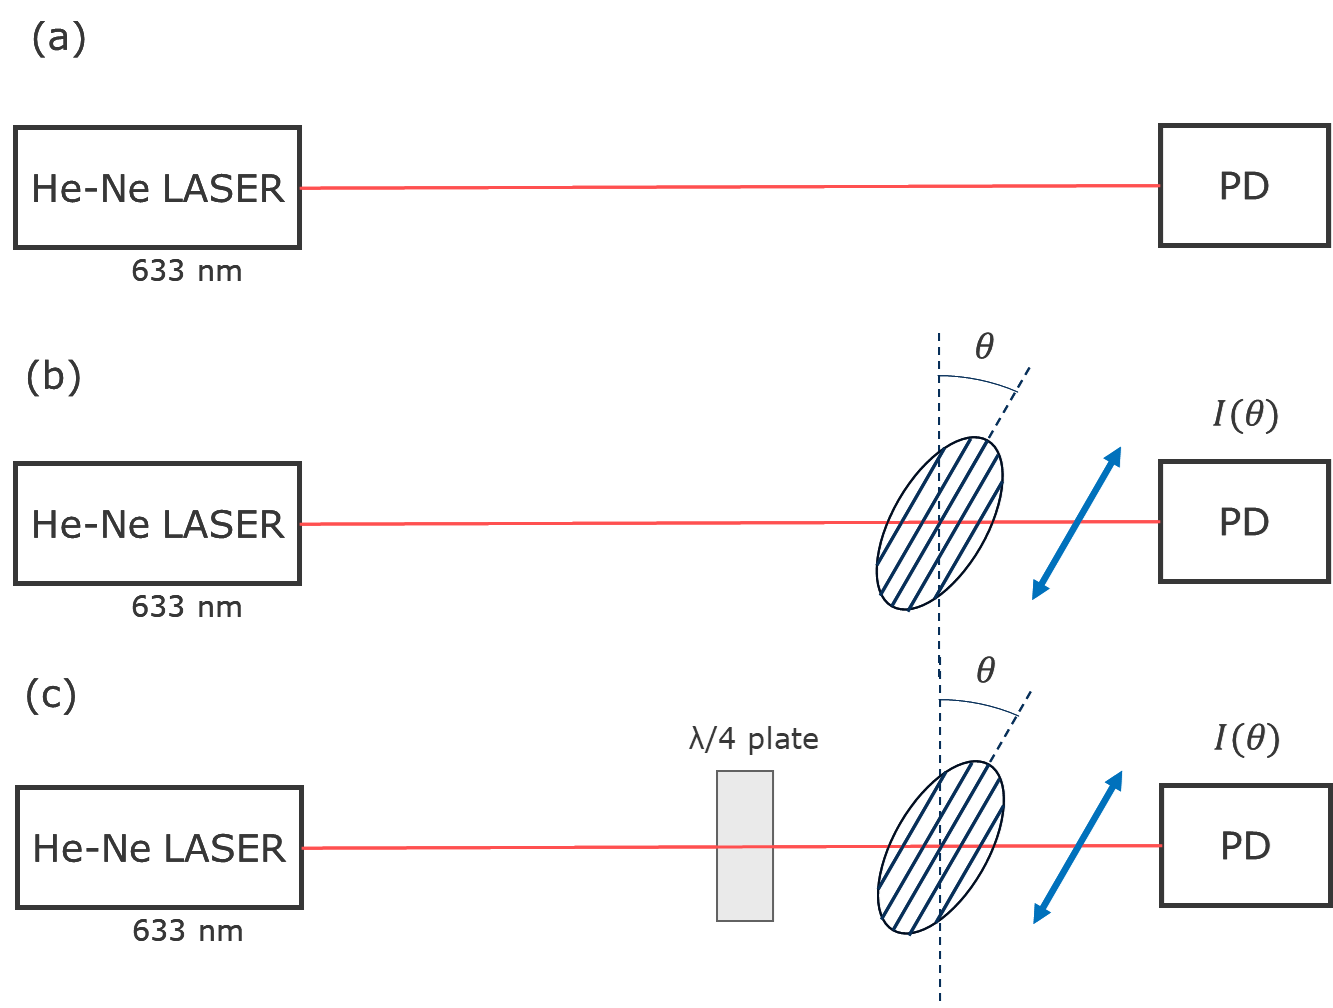
\includegraphics[width=0.48\columnwidth]{fig_ex-1.png}
    \caption{実験1: レーザー光の偏光の測定系}
    \label{fig:ex-1}
\end{wrapfigure}
レーザー光の偏光の性質をみるため、以下のような実験を行った。

はじめに、強度が安定しているかを確認するため、10 分間 He-Ne レーザー光の強度を1分おきに測定した(図\ref{fig:ex-1}-a)。
その後、レーザー光の偏光面の偏りを調べるため、図\ref{fig:ex-1}-b のように偏光板を追加して、
偏光板の角度を変えたときの強度の変化を測定した。
偏光板の特定の角度で光の強度が強くなるとしたら、
その角度がレーザー光の偏光面の傾きであると期待できる。
このように偏光面の角度を知る役割の偏光板を検光子と呼ぶ。

また、円偏光の度合を調べるため、\(\lambda/4\) 板を光路上に追加して、偏光版の角度を変えたときの強度の変化を測定した
(図\ref{fig:ex-1}-c)。
縦偏光と横偏光の位相差が \(\phi=\pm\pi/2\) に近く、円偏光のような形になっているとき、
\(\lambda/4\) 板を通すと直線偏光になるので、検光子の角度によって強度に変化が出ると予想される。

\section{結果・考察1: レーザー光の偏光}
レーザー光の強度は図\ref{graph:ex-1-1}のようになった。
光の強度はフォトダイオードの出力する値で 1.73 V で一定であるため、
以降の測定では光源は安定しているものとみなすことができる。

\begin{figure}[H]
    \centering
    \begin{minipage}[t]{0.48\columnwidth}
        \centering
        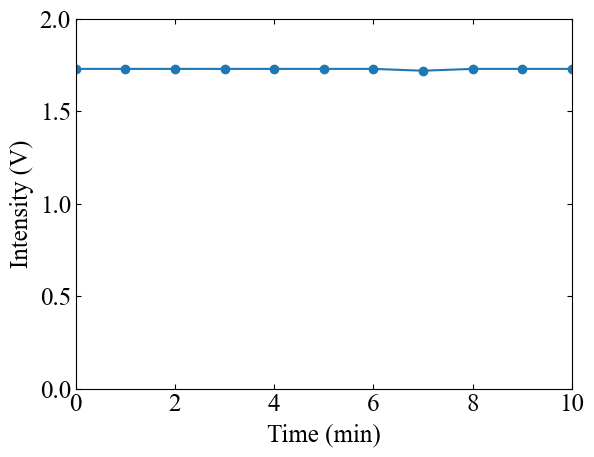
\includegraphics[width=\columnwidth]{11_29_00.png}
        \caption{光源の He-Ne レーザーの強度。縦軸はフォトダイオードの出力電圧。}
        \label{graph:ex-1-1}
    \end{minipage}
    \hfill
    \begin{minipage}[t]{0.48\columnwidth}
        \centering
        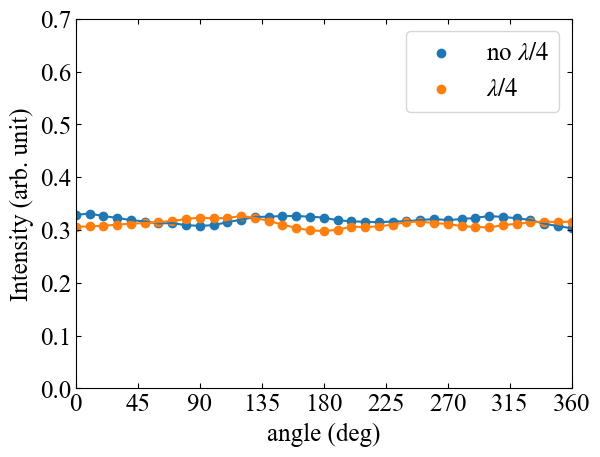
\includegraphics[width=\columnwidth]{11_29_01.png}
        \caption{レーザー光の偏光の様子。
        横軸は検光子の角度、縦軸は図\ref{graph:ex-1-1}の強度を基準とした強度。
        no \(\lambda/4\) は \(\lambda/4\) 板を通さず直接検光子を通したときの強度、
        \(\lambda/4\) は \(\lambda/4\) 板を通してから検光子を通したときの強度。}
        \label{graph:ex-1-2}
    \end{minipage}
\end{figure}

レーザー光の偏光の様子を測定するため、
検光子と \(\lambda/4\) 板を通した後の光の強度は図\ref{graph:ex-1-2}のようになった。
これを一般のジョーンズベクトル \(E = \,^t(\cos a,\,e^{ib}\sin a)\)を仮定した際に得られる強度の式とあわせて考える。
検光子のみ通したのときの強度は
\begin{align}
    I = &\cos^2 a \cos^4 \theta
    + 2 \cos a \cos b \cos^3 \theta \sin a \sin \theta
    + \cos^2 a \cos^2 \theta \sin^2 \theta \nonumber \\
    &+ \cos^2 b \cos^2 \theta \sin^2 a \sin^2 \theta
    + \cos^2 \theta \sin^2 a \sin^2 b \sin^2 \theta \nonumber \\
    &+ 2 \cos a \cos b \cos \theta \sin a \sin^3 \theta
    + \cos^2 b \sin^2 a \sin^4 \theta
    + \sin^2 a \sin^2 b \sin^4 \theta.
\end{align}
である。これを図\ref{graph:ex-1-2}と合うようにパラメータ \((a,b)\) を調整すると、\((a,b)=(\pi/4,\pi/2)\)となった。
これはレーザー光から出た直後の光が円偏光であることを表している。

一方、\(\lambda/4\) 板を通したときのジョーンズベクトルから計算したときの強度は
\begin{align}
    I =&\cos^2 a \cos^4 \theta
    - 2 \cos a \sin b \cos^3 \theta \sin a \sin \theta
    + \cos^2 a \cos^2 \theta \sin^2 \theta \nonumber \\
    &+ \sin^2 b \cos^2 \theta \sin^2 a \sin^2 \theta
    + \cos^2 b \cos^2 \theta \sin^2 a \sin^2 \theta \nonumber \\
    &- 2 \cos a \sin b \cos \theta \sin a \sin^3 \theta
    + \sin^2 b \sin^2 a \sin^4 \theta
    + \cos^2 b \sin^2 a \sin^4 \theta.
\end{align}
となる。
この式を図\ref{graph:ex-1-2}と合うようにパラメータ \((a,b)\) を調整すると、\((a,b)=(\pi/4,0)\)となった。
これはレーザー光から出た直後の光が直線偏光を表している。

ジョーンズベクトルを用いた解析では矛盾がでることから、
ジョーンズベクトルでの表記をする際に行った光の状態の仮定が誤っているのがわかる。
その仮定はレーザー光は特定の偏光の状態であるというものである。
よってレーザー光は非偏光であることがわかる。


\section{実験2: 直線偏光の取扱}
\begin{wrapfigure}{r}{0.48\columnwidth}
    \centering
    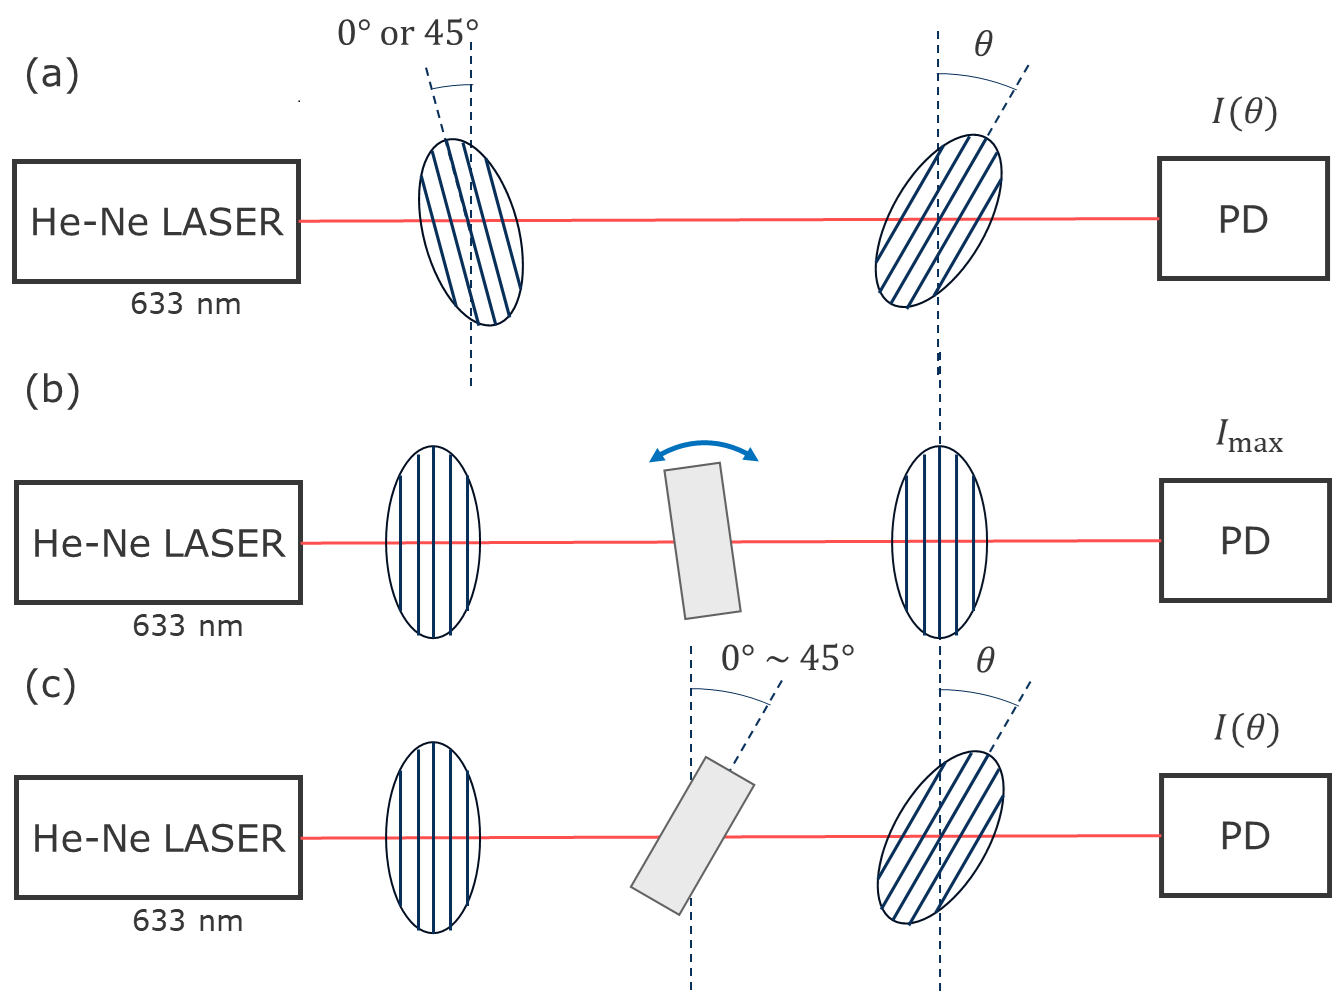
\includegraphics[width=0.48\columnwidth]{fig_ex-2.png}
    \caption{実験2: 直線偏光の取扱の測定系}
    \label{fig:ex-2}
\end{wrapfigure}
偏光板を通した後のレーザー光の性質を調べるため、以下のような実験を行った。

まずはじめに、レーザー光を通す偏光版の角度を \ang{0} と \ang{45}
\footnote{検光子の角度の方向と偏光子の角度の方向は逆向きになっている。} にし、
検光子を用いることでの偏光面の角度を調べた(図\ref{fig:ex-2}-a)。

次に、\(\lambda/4\) 板の規準となる角度を調べるため、
2つの偏光板の角度をあわせた後、
フォトダイオードの出力が最大となる角度に \(\lambda/4\) 板をセットした(図\ref{fig:ex-2}-b)。
この系をジョーンズ行列を用いて表すと、
\begin{align}
    \hat{J}(\theta) &= \hat{P}(0)\hat{Q}(\theta)\hat{P}(0) \notag\\
    &=\begin{pmatrix}
        \cos^2\theta + i\sin^2\theta  & 0\\
        0 & 0
    \end{pmatrix}
\end{align}
これに \(\vb*{E}=\,^t(E_{0x},E_{0y}e^{i\phi})\)の光が入ったときの光の強度は % TODO: 文章の流れを踏まえると実は論理が変
\begin{align}
    I(\theta) = \abs{\hat{J}(\theta)\vb*{E}}^2 \propto 1 -\frac{\sin^2 2\theta}{2}
\end{align}
となる。これの強度が最も強いときは \(\theta=0,\pi/2\)である。
\(\theta=0\) は縦偏光の位相を \(\pi/2\) 遅らせるもの、
\(\theta=\pi/2\) は横偏光の位相を \(\pi/2\) 進ませるものに対応し、
縦偏光と横変更の相対的な位相は変わらない。
なので最大となる\(\lambda/4\) 板の角度 \(\theta\) が2種類あるように見えるが、
どちらを選んだかわからなくても問題ないのがわかる。

その後、\(\lambda/4\) 板を規準となる角度から \ang{0}, \ang{15}, \ang{30}, \ang{45}
傾けたときの偏光面の角度を調べた(図\ref{fig:ex-2}-c)

\section{結果・考察2: 直線偏光の取扱}
レーザー光を通す偏光版の角度を \ang{0} と \ang{45} にしたときの測定結果は図\ref{graph:ex-2-1}のようになった。
これを見るとそれぞれの角度について
\begin{align}
    I_0(\theta) \propto \cos^2\theta,\qquad I_{45}(\theta) \propto \cos^2\qty(\theta + \frac{\pi}{4})
\end{align}
が成り立っているのがわかる(マリュス則)。
検光子のジョーンズ行列
\begin{align}
    \hat{P}(\theta) =
    \begin{pmatrix}
        \cos^2\theta & \cos\theta\sin\theta\\
        \cos\theta\sin\theta & \sin^2\theta
    \end{pmatrix}
\end{align}
を作用させてマリュス則が成り立つような偏光はそれぞれ
\begin{align}
    \vb*{E}_0 = \begin{pmatrix}
        1 \\ 0
    \end{pmatrix},\qquad
    \vb*{E}_{45} = \frac{1}{\sqrt{2}}\begin{pmatrix}
        1 \\ 1
    \end{pmatrix}
\end{align}
である。
ジョーンズ行列との積\(\hat{P}(\theta)\vb*{E}\)を計算すると
\begin{align}
    \hat{P}(\theta)\vb*{E}
    = \begin{pmatrix}
        \cos^2\theta & \cos\theta \sin\theta\\
        \cos\theta\sin\theta & \sin^2\theta
    \end{pmatrix}
    \begin{pmatrix}
        1 \\ 0
    \end{pmatrix}
    = \begin{pmatrix}
        \cos^2\theta \\ \cos\theta\sin\theta
    \end{pmatrix}
\end{align}
であり、これの強度は
\begin{align}
    I(\theta) = \cos^4\theta +\cos^2\theta\sin^2\theta = \cos^2\theta
\end{align}
確かにマリュス則と一致しているのがわかる(課題1)。

この結果より、レーザー光を偏光板に通すと直線偏光が得られることがわかった。

直線偏光を \(\lambda/4\) 板に通した時の偏光面の様子は図\ref{graph:ex-2-2}のようになった。
この系のジョーンズベクトルは
\begin{align}
    \hat{J}(\theta_1,\,\theta_2)\vb*{E} &= \hat{P}(\theta_2)\hat{Q}(\theta_1)\vb*{E}=
    \begin{pmatrix}
        \cos^2\theta_2 & \cos\theta_2\sin\theta_2\\
        \cos\theta_2\sin\theta_2 & \sin^2\theta_2
    \end{pmatrix}
    \begin{pmatrix}
        \cos^2\theta_1+i\sin^2\theta_1 & (1-i)\cos\theta_1\sin\theta_1\\
        (1-i)\cos\theta_1\sin\theta_1 & \sin^2\theta_1 + i \cos^2\theta_1
    \end{pmatrix}
    \begin{pmatrix}
        1\\0
    \end{pmatrix}\notag\\
    &=\begin{pmatrix}
        \cos^2(\theta_2) \left( \cos^2(\theta_1) + i \sin^2(\theta_1) \right) + \cos(\theta_2) \sin(\theta_2) \left( (1 - i) \cos(\theta_1) \sin(\theta_1) \right) \\
        \cos(\theta_2) \sin(\theta_2) \left( \cos^2(\theta_1) + i \sin^2(\theta_1) \right) + \sin^2(\theta_2) \left( (1 - i) \cos(\theta_1) \sin(\theta_1) \right)
    \end{pmatrix}
\end{align}
これより強度を計算すると
\begin{align}
    I(\theta_1,\,\theta_2) \propto \cos(4\theta_1-2\theta_2)+\cos(2\theta_2)+2
\end{align}
となる。これをグラフ描画ソフトで確認すると図\ref{graph:ex-2-2}とよく一致する。

これより、偏光が定まっているような光に対してはジョーンズベクトルによる方法はうまくいっているのがわかる。

\begin{figure}[H]
    \centering
    \begin{minipage}[t]{0.48\columnwidth}
        \centering
        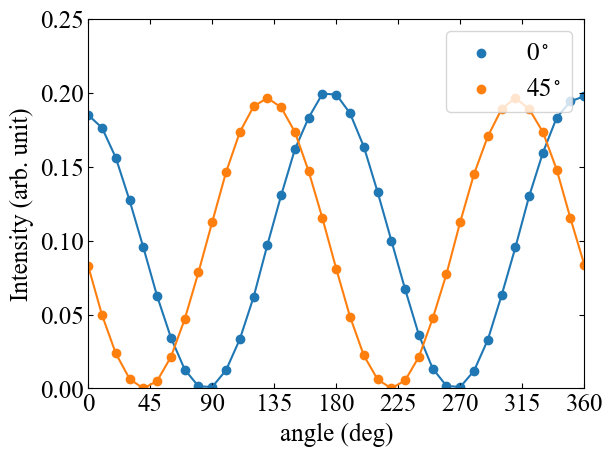
\includegraphics[width=\columnwidth]{11_29_02.png}
        \caption{偏光板を通した後のレーザー光の偏光の様子。
        横軸は検光子の角度、
        縦軸は図\ref{graph:ex-1-1}の強度を規準とした強度。
        凡例はレーザー光から出た後の偏光板の角度を表している。}
        \label{graph:ex-2-1}
    \end{minipage}
    \hfill
    \begin{minipage}[t]{0.48\columnwidth}
        \centering
        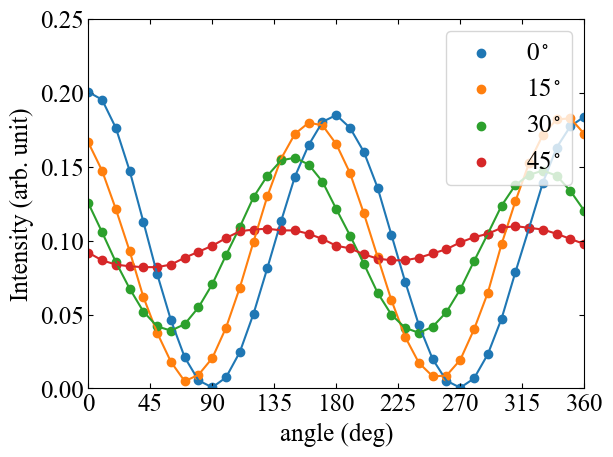
\includegraphics[width=\columnwidth]{11_29_03.png}
        \caption{偏光板を通した後のレーザー光(直線偏光)に \(\lambda/4\) 板を通したあとの偏光の様子。
        横軸は検光子の角度、
        縦軸は図\ref{graph:ex-1-1}の強度を規準とした強度。
        凡例は \(\lambda/4\) 板の角度を表している。}
        \label{graph:ex-2-2}
    \end{minipage}
\end{figure}

\section{実験3: ファラデー効果}
\begin{wrapfigure}{r}{0.48\columnwidth}
    \centering
    \caption{使用したソレノイドコイルのパラメータ}
    \label{table:ex-3}
    \begin{tabular}{rrrrr}
        \hline
        コイル & 巻き数 & 長さ (cm) & 直径 (cm) & 長岡係数\\
        \hline
        No.1 & 150 & 8.275 & 2.200 & 0.896\\
        No.2 & 100 & 7.238 & 2.200 & 0.882\\
        No.3 & 75 & 7.866 & 2.283 & 0.887\\
        No.4 & 50 & 7.478 & 2.200 & 0.886\\
        \hline
    \end{tabular}
\end{wrapfigure}

磁化のある媒質中を通った後の直線偏光の性質を調べるため、以下のような実験を行った。

測定する系は図\ref{fig:ex-3}の通りである。
偏光子を使って He-Ne レーザー光を直線偏光とし、
磁化を持った媒質を通って、偏光子と同じ角度にした検光子を通して強度を測定する。

偏光子と検光子を同じ角度にすることで、
媒質を通っても変化がないときには最も強い強度、変化があったときには強度が弱くなる。
これにより偏光の変化の様子を測定する。

磁化をもつ He-Ne レーザー光を透過する媒質として、
酸化テルビウムを含む磁気ガラスを使う。
これをソレノイドコイル中に通し、コイルに電流を流すことでテルビウムの磁化を誘起させる。
% 常磁性体であるため、磁化は
% \begin{align}
%     M = \chi H
% \end{align}
% というように単に比例するため磁場の強さによる偏光の違いを見る。

ソレノイドコイルは理想的な無限長さではないため、コイル内部の磁場は\(H=ni\)ではなく、
長岡係数\(K_n\)を用いて
\begin{gather}
    H = K_n n i\\
    K_n = \frac{4}{3\pi\sqrt{1-k^2}}\qty(\frac{1-k^2}{k^2}K(k)-\frac{1-2k^2}{k^2}E(k)-k),\qquad
    \frac{2r}{l} = \frac{k}{\sqrt{1-k^2}}
\end{gather}
というように補正される。
ここで、\(r\)はソレノイドコイルの半径、\(l\)はソレノイドコイルの軸方向の長さ、
\(K(k),\,E(k)\)はの第一種完全楕円積分および第二種完全楕円積分である。

このようなセッティングの元、4種類のコイル(表\ref{table:ex-3})を使い、
パルス電流の強さを変えて測定を行った。

次に、No.1 のコイルを使用して、偏光子の角度を \ang{45} にしたときの偏光の様子を測定した。
その後、パルス電流の流す向きを変えて同じ測定を行った。

\begin{figure}[H]
    \centering
    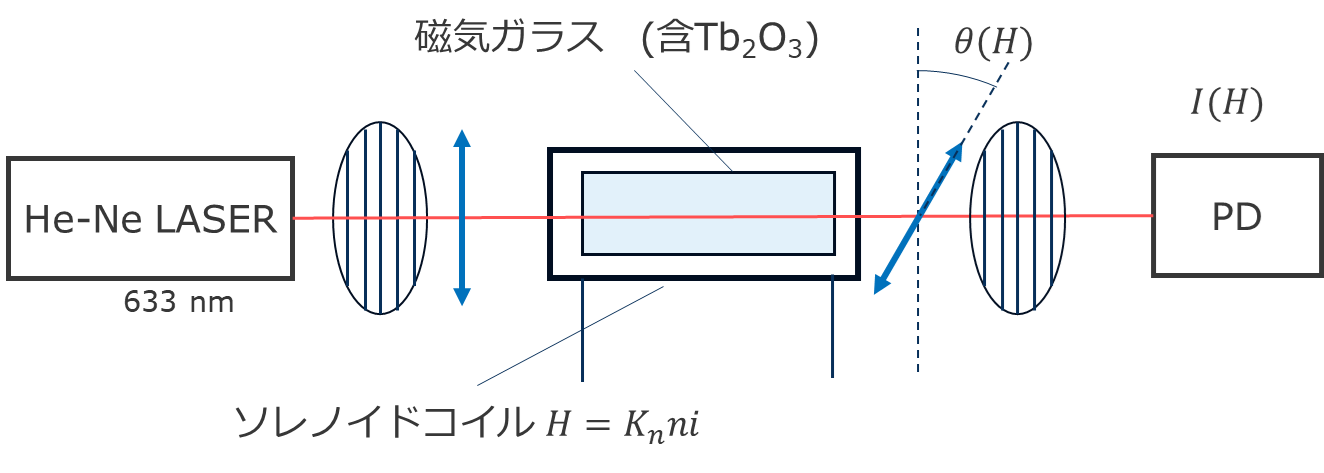
\includegraphics[width=0.7\columnwidth]{fig_ex-3.png}
    \caption{実験3: ファラデー効果の測定系}
    \label{fig:ex-3}
\end{figure}

\section{結果・考察3: ファラデー効果}
測定結果は以下のようになった。
ノイズをとるため実線は 5 次の Savitzky-Golay フィルターをかけたものを使った。

\ifodd1
\subsection*{x-t グラフ}
横軸に時間 (\si{\micro s})、左縦軸に透過光の強度 (arb. unit)、右縦軸に磁場の強さ (kA/cm) をプロットしたグラフは以下の通りである。
グラフの上部にあるのはソレノイドコイルの巻き数とパルス発生電流を装置の充電電圧である。

始めに偏光子と検光子のなす角度が 0 度のときの結果を示す。
\begin{figure}[H]
    \centering
    \begin{minipage}[t]{0.24\columnwidth}
        \centering
        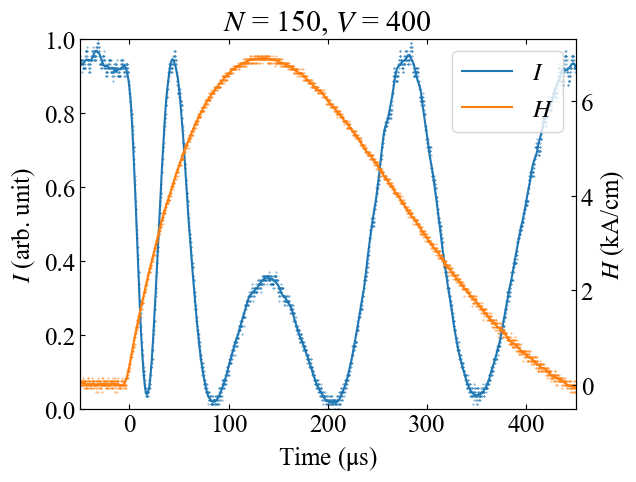
\includegraphics[width = \columnwidth]{xt/01.png}
    \end{minipage}
    \hfill
    \begin{minipage}[t]{0.24\columnwidth}
        \centering
        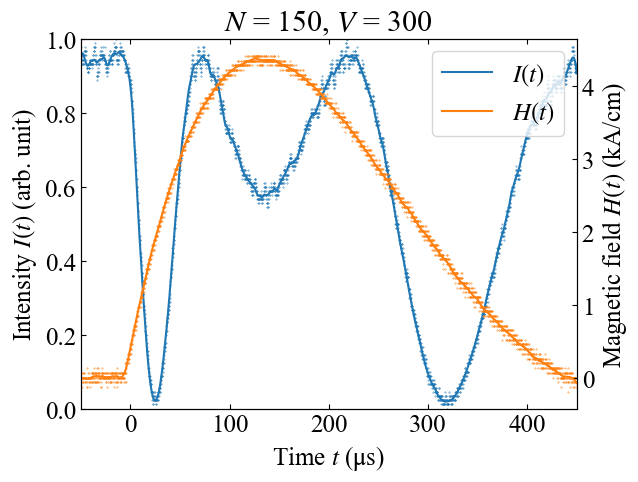
\includegraphics[width = \columnwidth]{xt/02.png}
    \end{minipage}
    \hfill
    \begin{minipage}[t]{0.24\columnwidth}
        \centering
        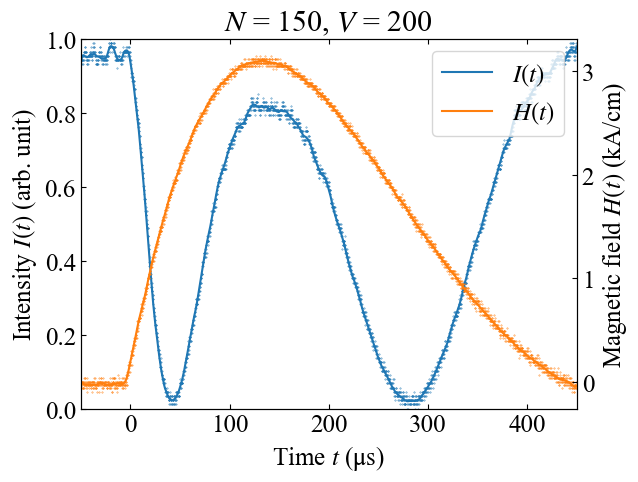
\includegraphics[width = \columnwidth]{xt/03.png}
    \end{minipage}
    \hfill
    \begin{minipage}[t]{0.24\columnwidth}
        \centering
        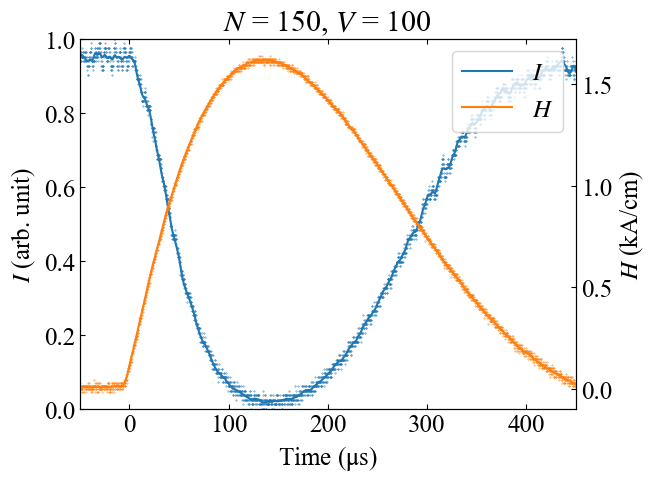
\includegraphics[width = \columnwidth]{xt/04.png}
    \end{minipage}
\end{figure}
\begin{figure}[H]
    \centering
    \begin{minipage}[t]{0.24\columnwidth}
        \centering
        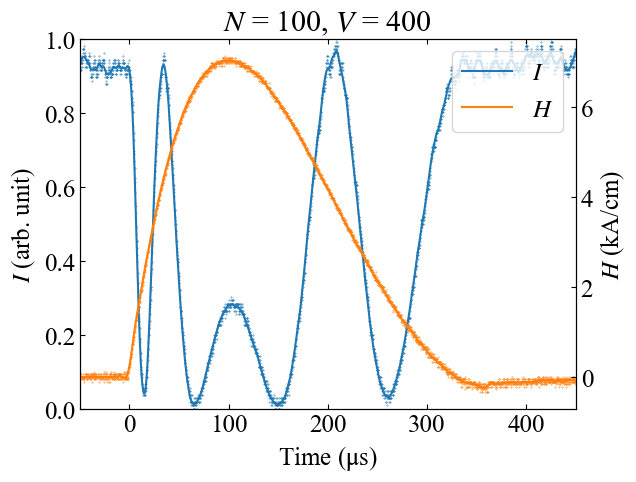
\includegraphics[width = \columnwidth]{xt/05.png}
    \end{minipage}
    \hfill
    \begin{minipage}[t]{0.24\columnwidth}
        \centering
        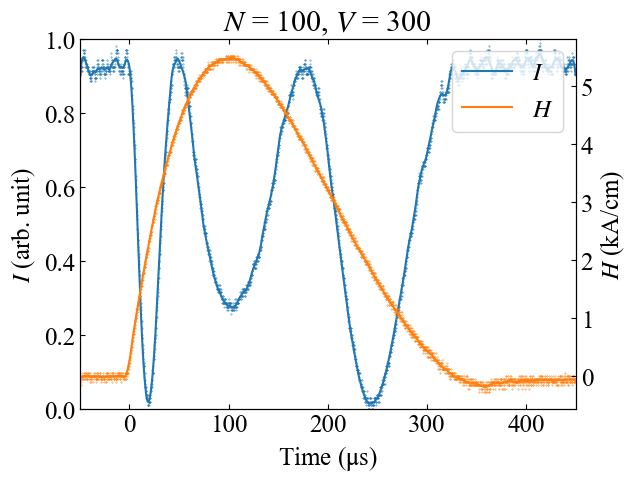
\includegraphics[width = \columnwidth]{xt/06.png}
    \end{minipage}
    \hfill
    \begin{minipage}[t]{0.24\columnwidth}
        \centering
        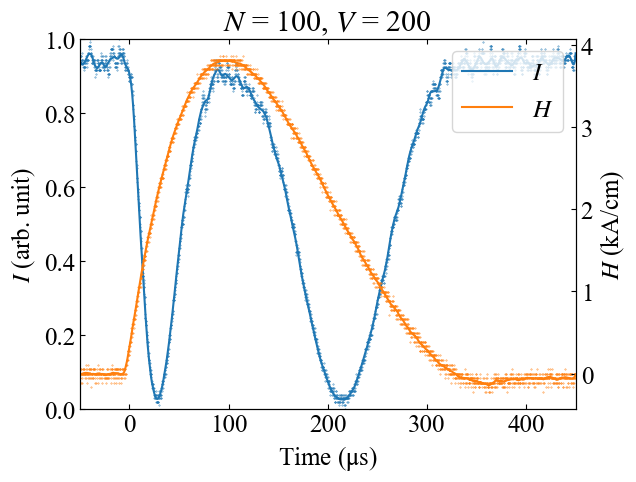
\includegraphics[width = \columnwidth]{xt/07.png}
    \end{minipage}
    \hfill
    \begin{minipage}[t]{0.24\columnwidth}
        \centering
        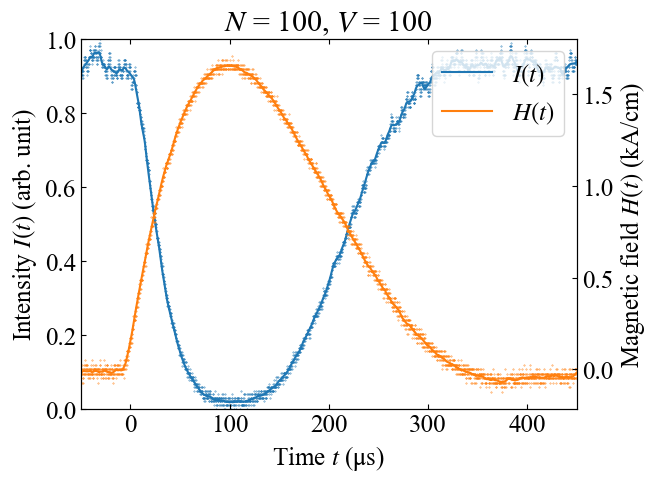
\includegraphics[width = \columnwidth]{xt/08.png}
    \end{minipage}
\end{figure}
\begin{figure}[H]
    \centering
    \begin{minipage}[t]{0.24\columnwidth}
        \centering
        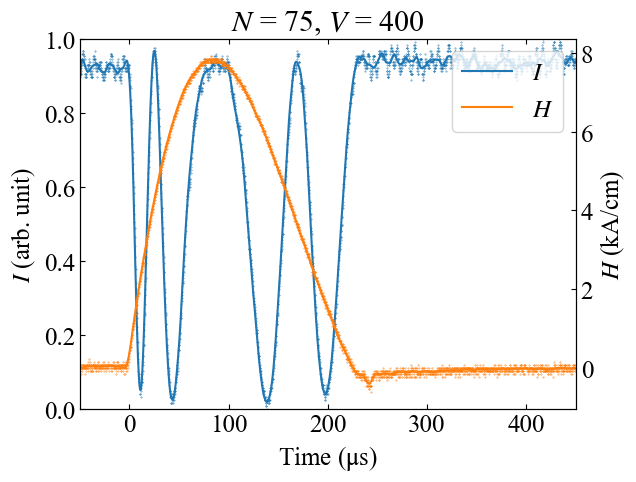
\includegraphics[width = \columnwidth]{xt/09.png}
    \end{minipage}
    \hfill
    \begin{minipage}[t]{0.24\columnwidth}
        \centering
        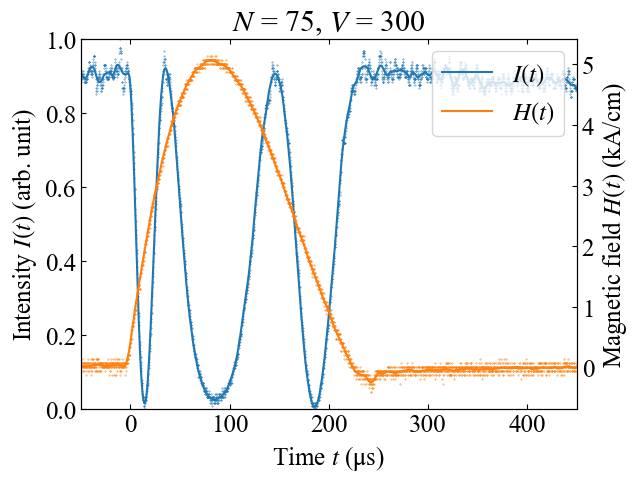
\includegraphics[width = \columnwidth]{xt/10.png}
    \end{minipage}
    \hfill
    \begin{minipage}[t]{0.24\columnwidth}
        \centering
        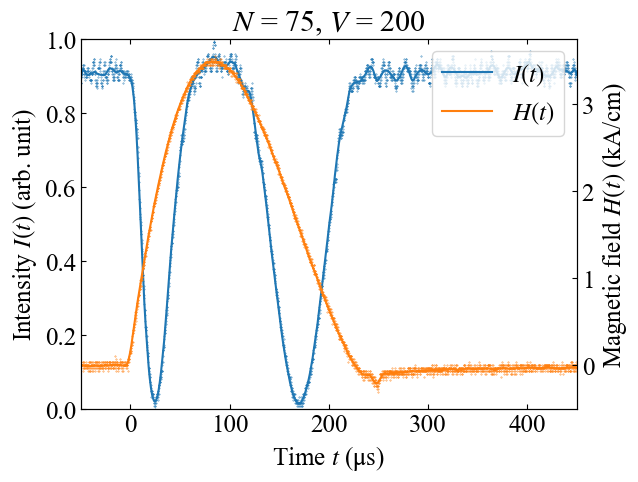
\includegraphics[width = \columnwidth]{xt/11.png}
    \end{minipage}
    \hfill
    \begin{minipage}[t]{0.24\columnwidth}
        \centering
        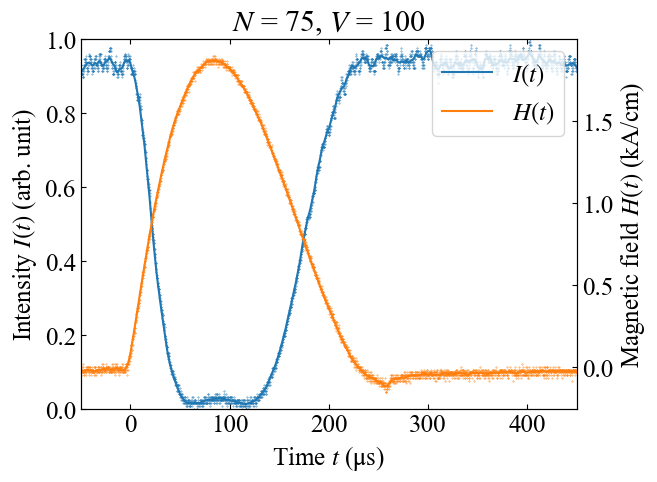
\includegraphics[width = \columnwidth]{xt/12.png}
    \end{minipage}
\end{figure}
\begin{figure}[H]
    \centering
    \begin{minipage}[t]{0.24\columnwidth}
        \centering
        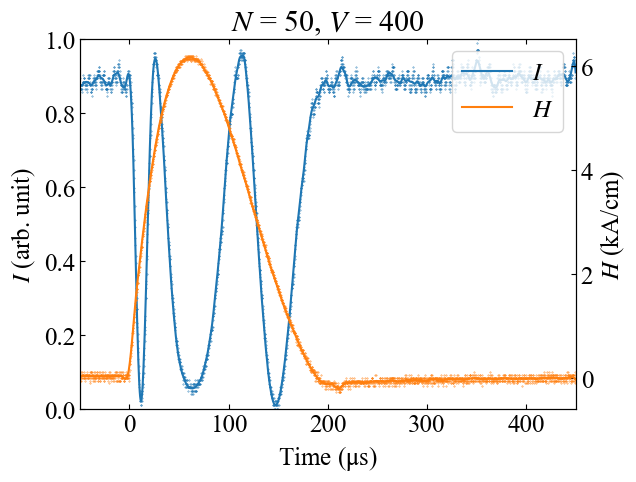
\includegraphics[width = \columnwidth]{xt/13.png}
    \end{minipage}
    \hfill
    \begin{minipage}[t]{0.24\columnwidth}
        \centering
        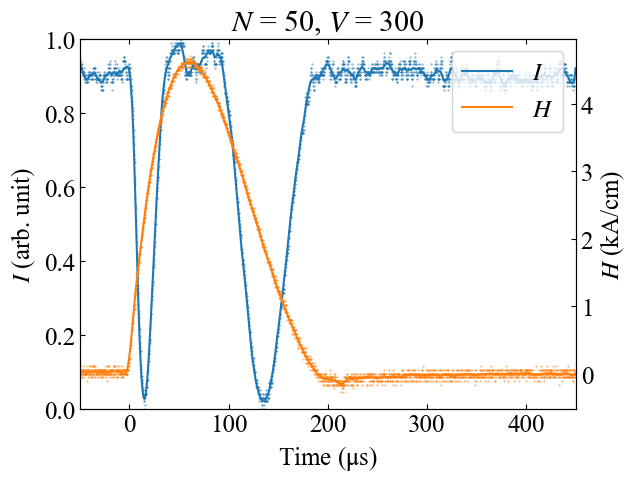
\includegraphics[width = \columnwidth]{xt/14.png}
    \end{minipage}
    \hfill
    \begin{minipage}[t]{0.24\columnwidth}
        \centering
        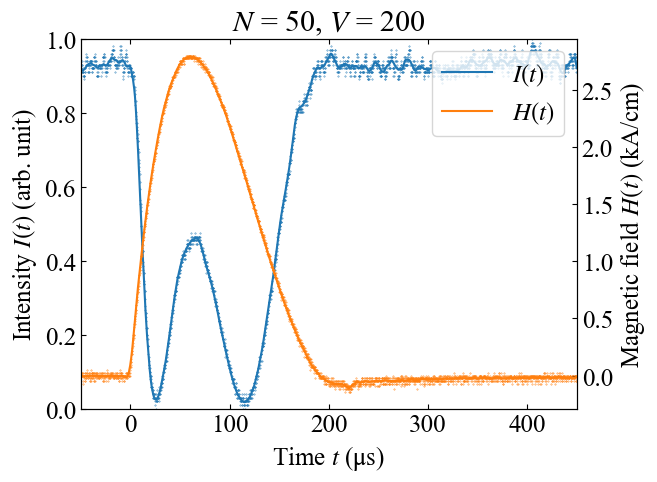
\includegraphics[width = \columnwidth]{xt/15.png}
    \end{minipage}
    \hfill
    \begin{minipage}[t]{0.24\columnwidth}
        \centering
        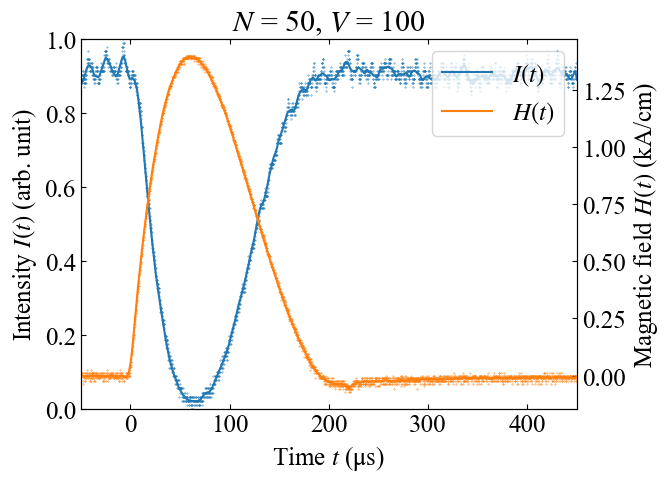
\includegraphics[width = \columnwidth]{xt/16.png}
    \end{minipage}
\end{figure}

次に偏光子と検光子のなす角度が 45 度のときの結果を示す。
\begin{figure}[H]
    \centering
    \begin{minipage}[t]{0.24\columnwidth}
        \centering
        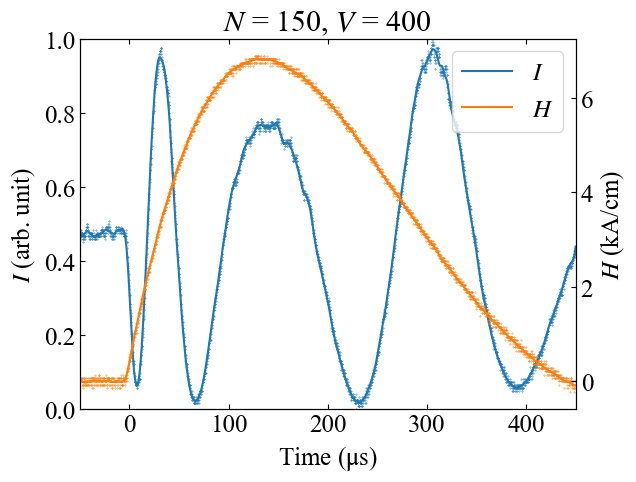
\includegraphics[width = \columnwidth]{xt/17.png}
    \end{minipage}
    \hfill
    \begin{minipage}[t]{0.24\columnwidth}
        \centering
        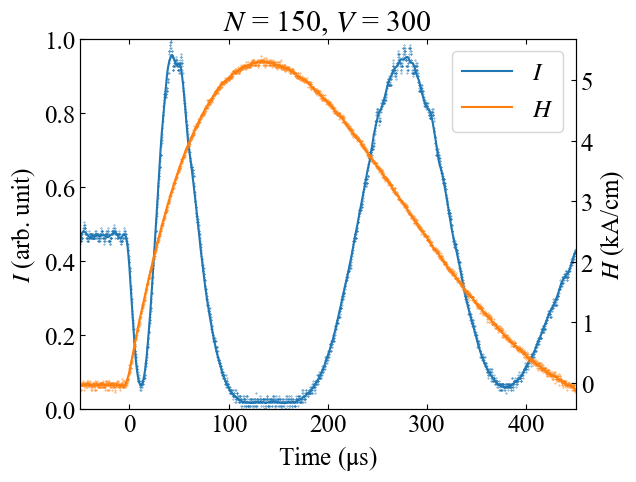
\includegraphics[width = \columnwidth]{xt/18.png}
    \end{minipage}
    \hfill
    \begin{minipage}[t]{0.24\columnwidth}
        \centering
        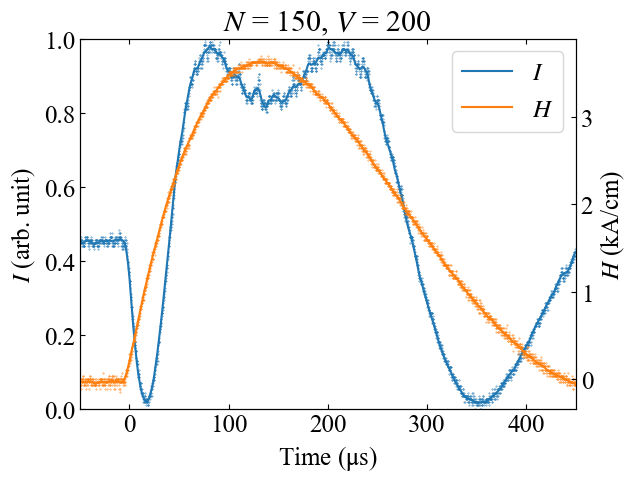
\includegraphics[width = \columnwidth]{xt/19.png}
    \end{minipage}
    \hfill
    \begin{minipage}[t]{0.24\columnwidth}
        \centering
        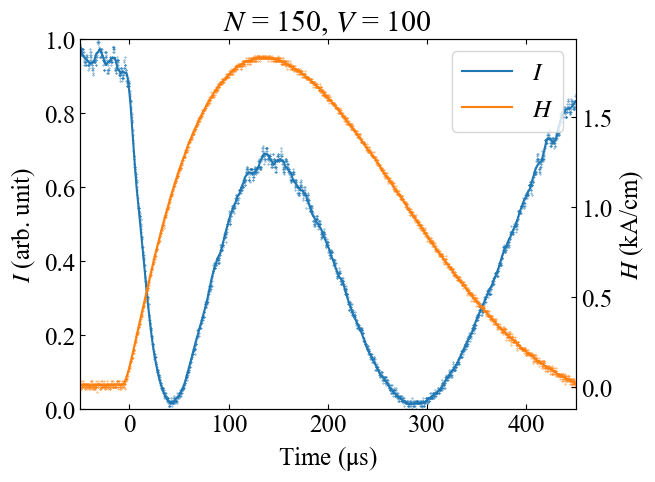
\includegraphics[width = \columnwidth]{xt/20.png}
    \end{minipage}
\end{figure}

最後にパルス電流の向きを変えることで磁場の向きを今までの向きとは反平行にして、偏光子と検光子のなす角度が 45 度のときの結果を示す。
\begin{figure}[H]
    \centering
    \begin{minipage}[t]{0.24\columnwidth}
        \centering
        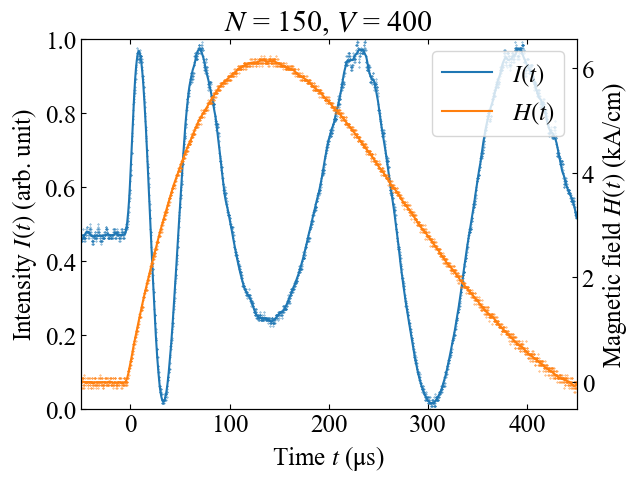
\includegraphics[width = \columnwidth]{xt/22.png}
    \end{minipage}
    \hfill
    \begin{minipage}[t]{0.24\columnwidth}
        \centering
        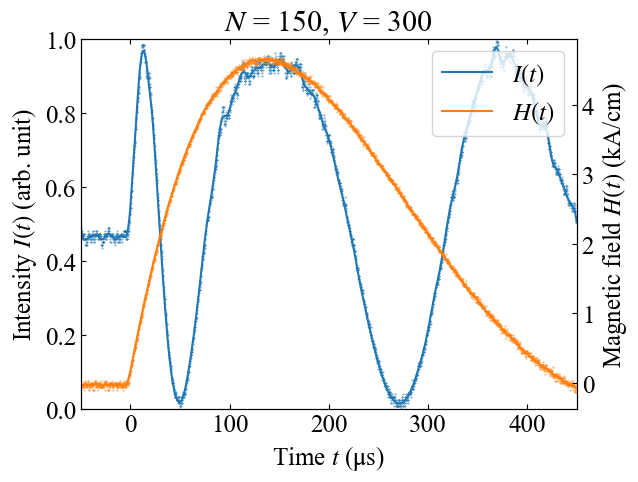
\includegraphics[width = \columnwidth]{xt/23.png}
    \end{minipage}
    \hfill
    \begin{minipage}[t]{0.24\columnwidth}
        \centering
        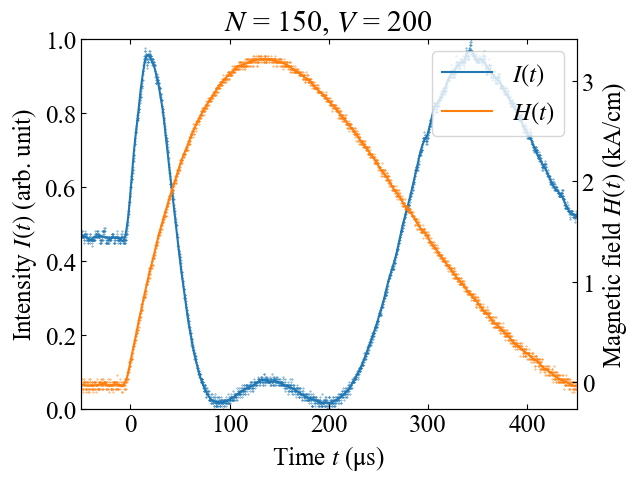
\includegraphics[width = \columnwidth]{xt/24.png}
    \end{minipage}
    \hfill
    \begin{minipage}[t]{0.24\columnwidth}
        \centering
        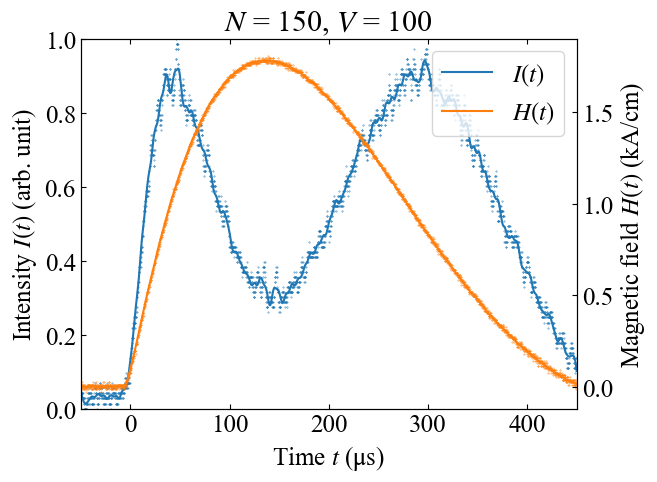
\includegraphics[width = \columnwidth]{xt/25.png}
    \end{minipage}
\end{figure}

\subsection*{x-y グラフ}

横軸に磁場の強さ (kA/cm)、縦軸に透過光の強度 (arb. unit) をプロットしたグラフは以下の通りである。
磁場による磁気ガラス中の磁化の応答が遅れるがあるため、
それを補正したものと補正していないもの両方を載せる。

補正はこのようにして行った。
磁場の強さと透過光の強度の x-y グラフを作る際に、
時刻\(t[i]\)のときの磁場の強さと透過光を\(H[i], I[i]\)というようにおく。
磁化の応答が遅れるということは、同じだけ透過光の応答も遅らせればよい。
なので
\begin{align}
    (H[i], I[i+\text{shift}])
\end{align}
というように光強度も shift の分だけ遅らせたペアの点をプロットするというようにして補正した。

グラフの上部にあるのはソレノイドコイルの巻き数とパルス発生装置の充電電圧、どれだけシフトしたかの量である。

始めに偏光子と検光子のなす角度が 0 度のときの結果を示す。
\begin{figure}[H]
    \centering
    \begin{minipage}[t]{0.24\columnwidth}
        \centering
        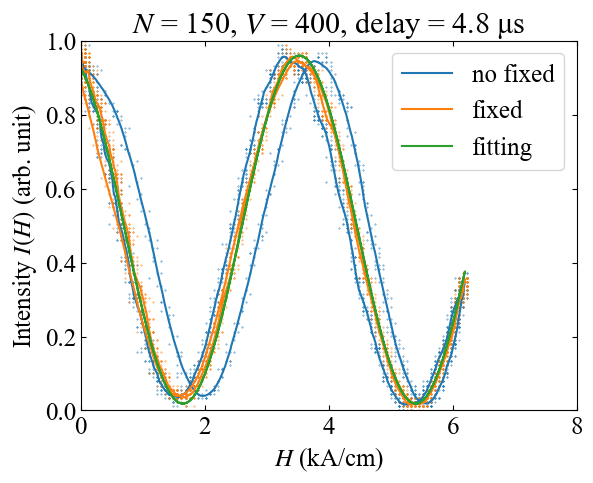
\includegraphics[width = \columnwidth]{xy/01.png}
    \end{minipage}
    \hfill
    \begin{minipage}[t]{0.24\columnwidth}
        \centering
        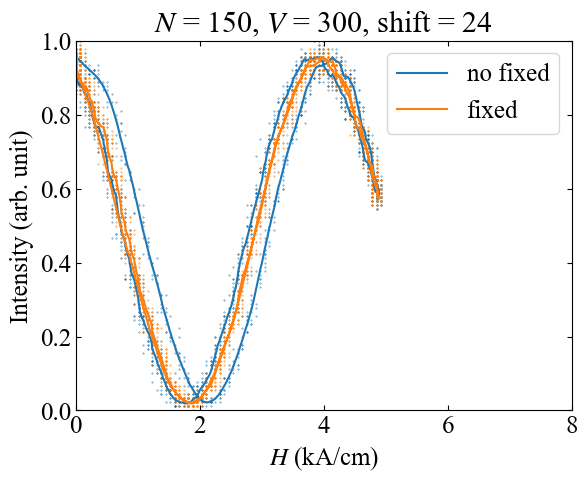
\includegraphics[width = \columnwidth]{xy/02.png}
    \end{minipage}
    \hfill
    \begin{minipage}[t]{0.24\columnwidth}
        \centering
        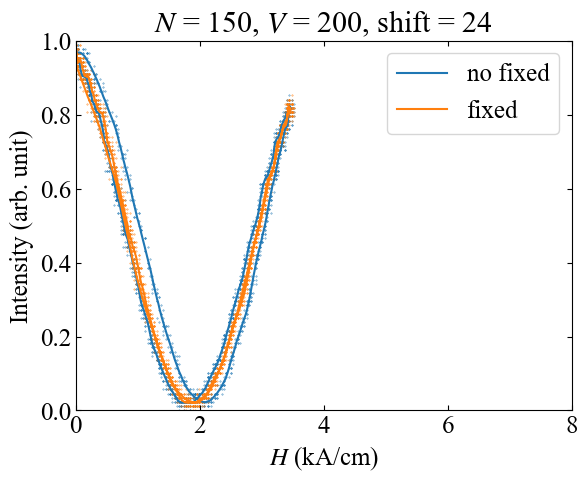
\includegraphics[width = \columnwidth]{xy/03.png}
    \end{minipage}
    \hfill
    \begin{minipage}[t]{0.24\columnwidth}
        \centering
        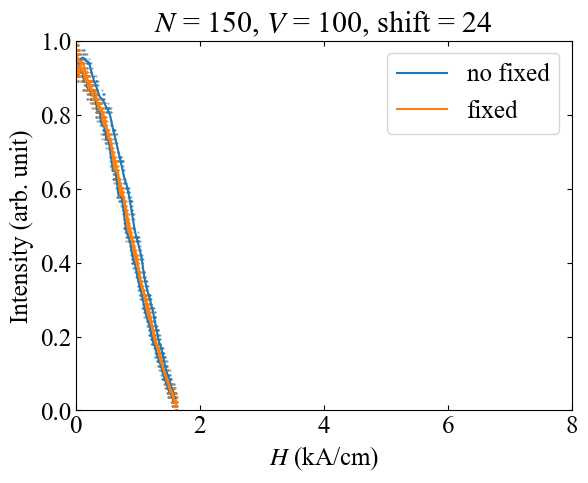
\includegraphics[width = \columnwidth]{xy/04.png}
    \end{minipage}
\end{figure}
\begin{figure}[H]
    \centering
    \begin{minipage}[t]{0.24\columnwidth}
        \centering
        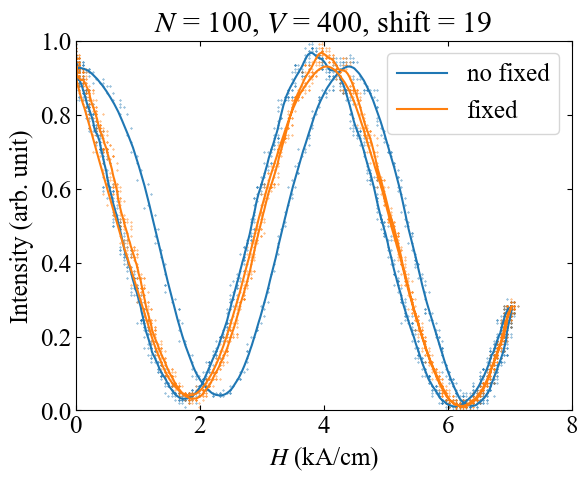
\includegraphics[width = \columnwidth]{xy/05.png}
    \end{minipage}
    \hfill
    \begin{minipage}[t]{0.24\columnwidth}
        \centering
        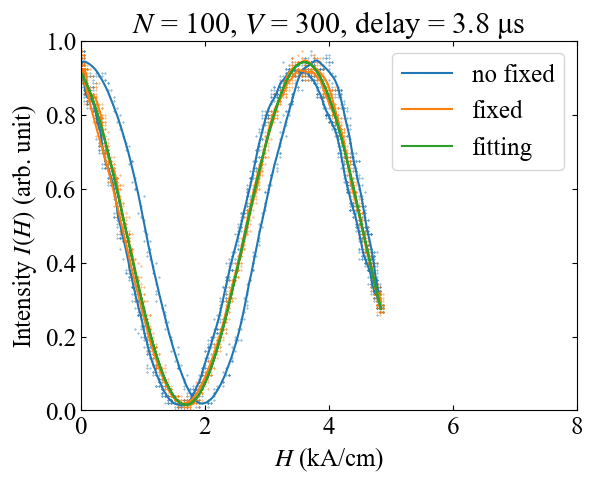
\includegraphics[width = \columnwidth]{xy/06.png}
    \end{minipage}
    \hfill
    \begin{minipage}[t]{0.24\columnwidth}
        \centering
        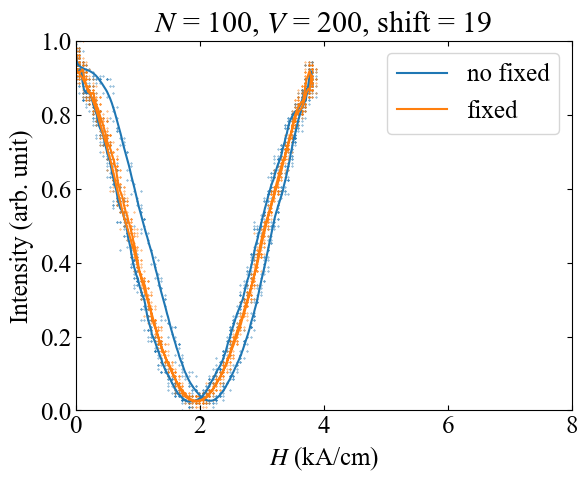
\includegraphics[width = \columnwidth]{xy/07.png}
    \end{minipage}
    \hfill
    \begin{minipage}[t]{0.24\columnwidth}
        \centering
        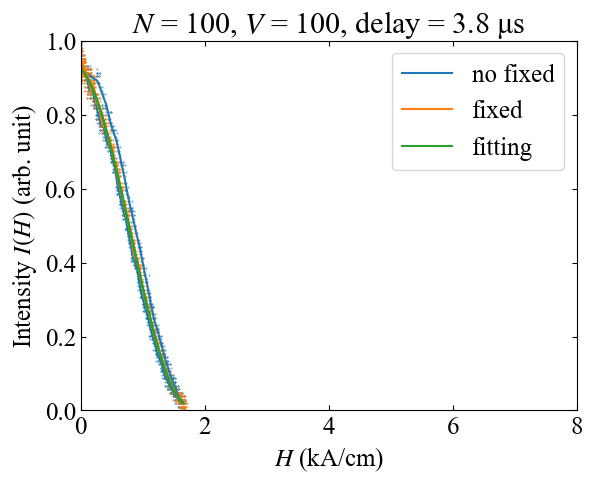
\includegraphics[width = \columnwidth]{xy/08.png}
    \end{minipage}
\end{figure}
\begin{figure}[H]
    \centering
    \begin{minipage}[t]{0.24\columnwidth}
        \centering
        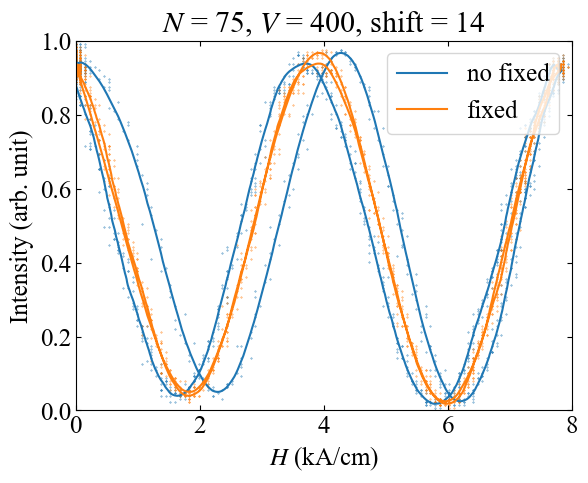
\includegraphics[width = \columnwidth]{xy/09.png}
    \end{minipage}
    \hfill
    \begin{minipage}[t]{0.24\columnwidth}
        \centering
        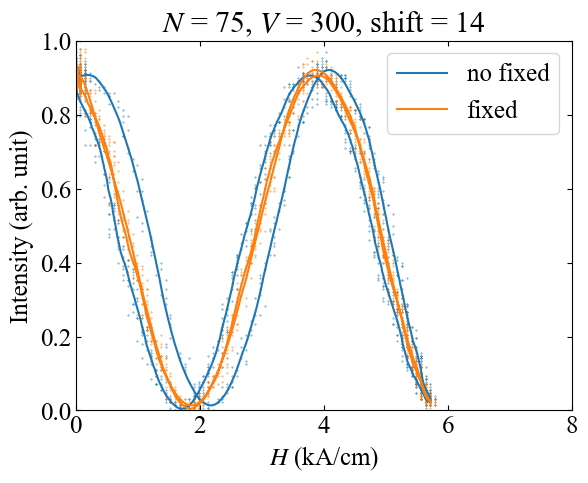
\includegraphics[width = \columnwidth]{xy/10.png}
    \end{minipage}
    \hfill
    \begin{minipage}[t]{0.24\columnwidth}
        \centering
        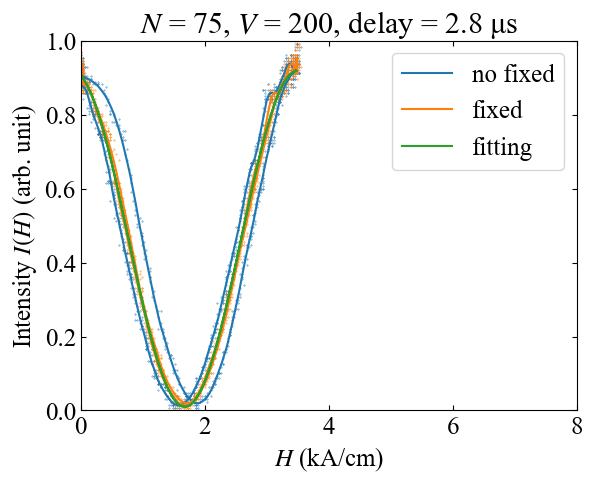
\includegraphics[width = \columnwidth]{xy/11.png}
    \end{minipage}
    \hfill
    \begin{minipage}[t]{0.24\columnwidth}
        \centering
        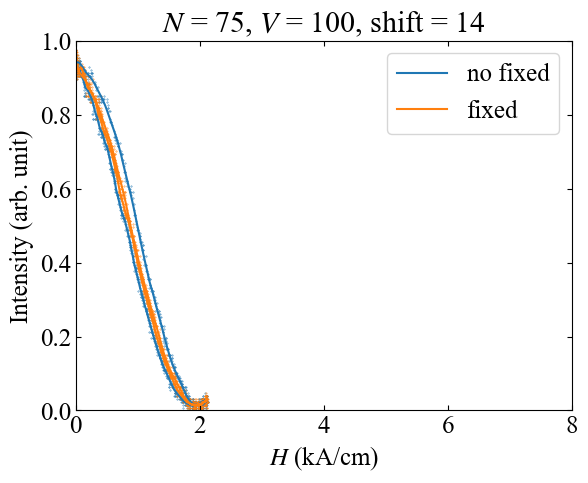
\includegraphics[width = \columnwidth]{xy/12.png}
    \end{minipage}
\end{figure}
\begin{figure}[H]
    \centering
    \begin{minipage}[t]{0.24\columnwidth}
        \centering
        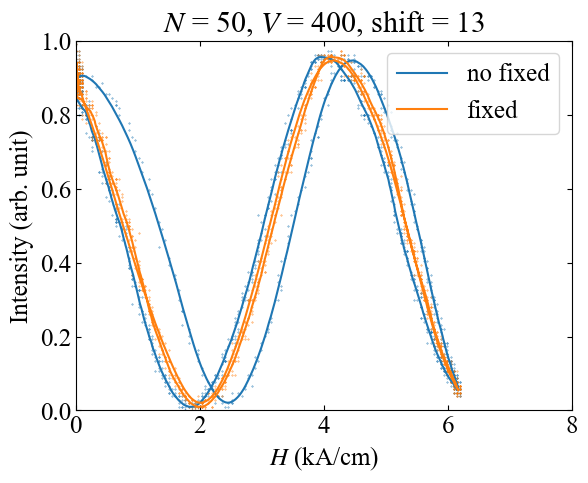
\includegraphics[width = \columnwidth]{xy/13.png}
    \end{minipage}
    \hfill
    \begin{minipage}[t]{0.24\columnwidth}
        \centering
        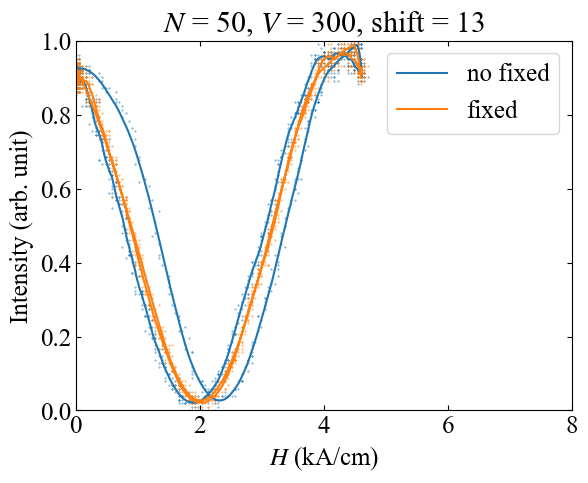
\includegraphics[width = \columnwidth]{xy/14.png}
    \end{minipage}
    \hfill
    \begin{minipage}[t]{0.24\columnwidth}
        \centering
        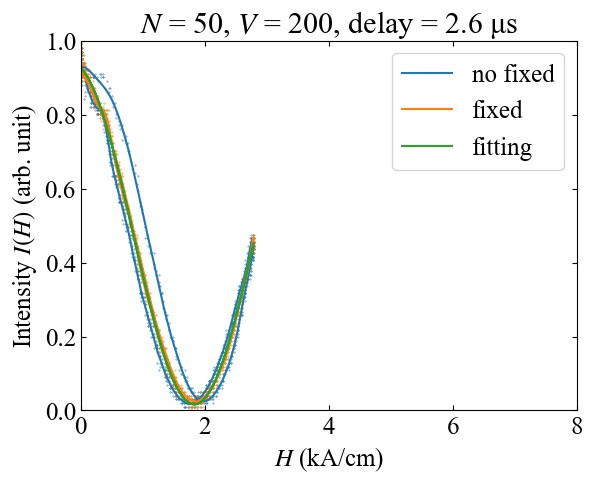
\includegraphics[width = \columnwidth]{xy/15.png}
    \end{minipage}
    \hfill
    \begin{minipage}[t]{0.24\columnwidth}
        \centering
        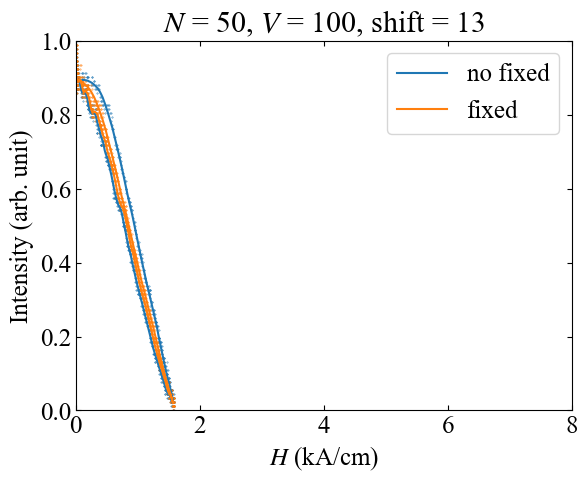
\includegraphics[width = \columnwidth]{xy/16.png}
    \end{minipage}
\end{figure}

次に偏光子と検光子のなす角度が 45 度のときの結果を示す。
\begin{figure}[H]
    \centering
    \begin{minipage}[t]{0.24\columnwidth}
        \centering
        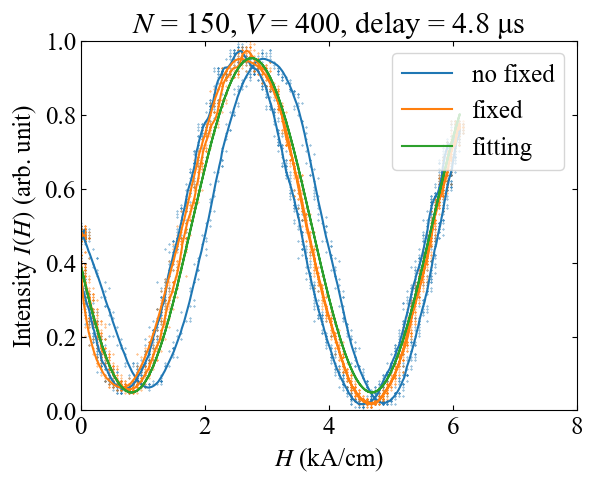
\includegraphics[width = \columnwidth]{xy/17.png}
    \end{minipage}
    \hfill
    \begin{minipage}[t]{0.24\columnwidth}
        \centering
        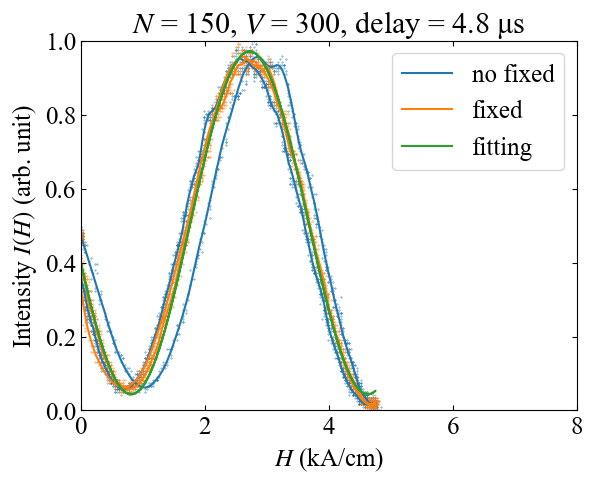
\includegraphics[width = \columnwidth]{xy/18.png}
    \end{minipage}
    \hfill
    \begin{minipage}[t]{0.24\columnwidth}
        \centering
        \includegraphics[width = \columnwidth]{xy/19.png}
    \end{minipage}
    \hfill
    \begin{minipage}[t]{0.24\columnwidth}
        \centering
        \includegraphics[width = \columnwidth]{xy/20.png}
    \end{minipage}
\end{figure}

最後にパルス電流の向きを変えることで磁場の向きを今までの向きとは反平行にして、偏光子と検光子のなす角度が 45 度のときの結果を示す。
\begin{figure}[H]
    \centering
    \begin{minipage}[t]{0.24\columnwidth}
        \centering
        \includegraphics[width = \columnwidth]{xy/22.png}
    \end{minipage}
    \hfill
    \begin{minipage}[t]{0.24\columnwidth}
        \centering
        \includegraphics[width = \columnwidth]{xy/23.png}
    \end{minipage}
    \hfill
    \begin{minipage}[t]{0.24\columnwidth}
        \centering
        \includegraphics[width = \columnwidth]{xy/24.png}
    \end{minipage}
    \hfill
    \begin{minipage}[t]{0.24\columnwidth}
        \centering
        \includegraphics[width = \columnwidth]{xy/25.png}
    \end{minipage}
\end{figure}
\clearpage
\fi
\begin{wrapfigure}{r}{0.48\columnwidth}
    \centering
    \includegraphics[width=0.48\columnwidth]{verdet.png}
    \caption{実験3: ファラデー効果の測定結果から得られたベルデ定数}
    \label{graph:ex-3-1}
\end{wrapfigure}
偏光子を掛けていないときの x-y グラフから、
強度と磁場の間には比例定数ある定数を \(a\) として
\begin{align}
    I(H) \propto \cos^2 aH
\end{align}
というように書けるのがわかる。
これは図\ref{fig:ex-2}-a での結果であるマリュス則と同じ形となっている。
つまり、磁化がある媒質中を直線偏光が通ると、
直線偏光の偏光面の角度が磁場に比例して変わるということを表している(ファラデー効果)。
この結果は偏光子の角度を \ang{45} つけたときには \(I \propto \cos^2(aH+\pi/4)\) になっていることや、
さらに磁場の向きを逆向きにしたときには \(I \propto \cos^2(-aH+\pi/4)\) となっていることからもわかる。

磁気ガラスの長さが長ければ、光が媒質中を滞在する時間が増え、磁化との相互作用が多くなる。
なのでこの定数を長さで割った量(ベルデ定数)というのが、物質固有の量であると考えられる。
磁気ガラスの長さを 5.00 cm として、比例定数 \(a\) をこれらのグラフから \(I(H) \propto \cos^2 aH+b\)でフィッティングすることで求めると、
図\ref{graph:ex-3-1}のようになった。

各実験から得られたベルデ定数の平均値は 9.63 deg/kA であった。
長岡係数による補正があるものの、実験テキストにある文献値 1.04 deg/kA とはずれてしまった。
このずれは実際に測定をしていない磁気ガラスの長さが正確ではないと違うといったことが考えられる。
文献値のベルデ定数があっているものとして、これをもとに磁気ガラスの長さを求めると 4.63 cm である。
4 mm のずれは考えにくいので、他にも要因があるように考えられる。

\begin{wrapfigure}{r}{0.28\columnwidth}
    \centering
    \caption{実験3: 外部磁場に対する磁気ガラス中の磁化の応答の遅れ}
    \label{table:ex-3-1}
    \begin{tabular}{rr}
        \hline
        コイル & 遅れ (\si{\micro s})\\
        \hline
        No.1 & 4.8\\
        No.2 & 3.8\\
        No.3 & 2.8\\
        No.4 & 2.6\\
        \hline
    \end{tabular}
\end{wrapfigure}
他に挙げられる原因として、磁気ガラス中の酸化テルビウムの量が文献値が測定したサンプルと異なるのも考えられる。
ベルデ定数が文献値より小さいことから、
今回測定した試料は磁気ガラス中の酸化テルビウムの量が文献値が測定した試料に比べ小さいと推測される。

また、x-y グラフを作る際に必要な磁場に対する磁化の応答の遅れを補正するためのシフト量は、
磁場の強さではなく、コイルの種類に関係していた(表\ref{table:ex-3-1})。
これの解釈は正直わからない。
有限長のソレノイドコイルであることや、
コイルの巻きむらによって、コイル中の磁場が不均一となるため、
磁気ガラスの配置に敏感に影響されたのではないかと考えている。

\section{課題}
\begin{tcolorbox}[colbacktitle=white, coltitle=black, colback=white, title = 課題1]
    直線偏光の光が偏光板を透過した時、その透過光強度 \(I\) は
    \begin{align*}
        I(\theta) = I_0 \cos^2\theta
    \end{align*}
    となることを説明せよ。ここで、\(I_0\) は偏光板への入射光強度、
    \(\theta\) は電場方向と偏光板の透過軸の成す角であり、
    偏光板による吸収や反射は無視する。
\end{tcolorbox}

結果・考察2: 直線偏光の取扱で論じた。\\
\clearpage
\begin{tcolorbox}[colbacktitle=white, coltitle=black, colback=white, title = 課題2]
    光の偏光状態を表す手法として極座標表示がある。
    \(\lambda/4\) 板の特性を調べたときに得た偏光の実験結果を極座標表示で表しなさい。
\end{tcolorbox}
\begin{wrapfigure}{r}{0.45\columnwidth}
    \centering
    \includegraphics[width = 0.45 \columnwidth]{11_29_04.png}
    \caption{\(\lambda/4\) 板の特性を調べたときに得た偏光の実験結果(図\ref{graph:ex-2-2})の極座標表示。}
    \label{graph:ex-2-3}
\end{wrapfigure}
極座標表示で\(\lambda/4\) 板の特性を調べたときに得た偏光の実験結果(図\ref{graph:ex-2-2})を
プロットすると図\ref{graph:ex-2-3}のようになった。

これを見ると \(\lambda/4\) 板の角度が \ang{0} で直線偏光を変えないときには、
\(I(\theta)\propto\cos^2\theta\)に従って節があるような曲線となっている。
\(\lambda/4\) 板の角度を \ang{15}, \ang{30}, \ang{45} とつけていくと、
その角度にあわせて偏光面も \ang{15}, \ang{30}, \ang{45} と回転していくのがわかる。
これは \(\lambda/4\) 板のジョーンズ行列が
\begin{align}
    \hat{Q}(\theta)
    &=i\hat{I} + (1-i)\begin{pmatrix}
        \cos^2 \theta & \cos\theta\sin\theta\\
        \cos\theta\sin\theta & \sin^2\theta
    \end{pmatrix}\notag\\
    &=i\hat{I} + (1-i)\hat{P}(\theta)
\end{align}
というように偏光板のジョーンズ行列\(\hat{P}(\theta)\)を使って書くことができるのに対応している。
つまり、右辺第二項を反映して偏光面が回転していっていると解釈できる。

単位行列とのアフィン結合に虚数が入るため、
単に回転をするだけではなく節が消え、円周状になっていく。\\ \\

\begin{tcolorbox}[colbacktitle=white, coltitle=black, colback=white, title = 課題3]
    ファラデー効果の応用について調査せよ。また、その原理について説明せよ。
\end{tcolorbox}
光通信網のデバイスである光アイソレーターに使われる。

光通信の光源は半導体レーザーである。
半導体レーザー素子内部で発振して出た光は光ファイバーを通って回路網に流れていく。
こうした回路網の中での反射により、光が半導体レーザー素子に戻ってくることがある。
するとレーザー発振が不安定になり、信号の室が悪くなる。
こうした影響をなくすため、戻ってくる光のみを遮断するような部品が必要となる。
これを光アイソレーターという。

図\ref{fig:assignment-1}はファラデー効果の使った光アイソレーターの模式図である。
半導体レーザーから出た光を偏光板に通し直線偏光にしたあと、
ファラデー効果を用いて、偏光面を \ang{45} 回転させる。
そして同じく \ang{45} 回転させた偏光板に通して回路につなぐといったものである。
このようにすると光源から出る光は直線偏光にするところ以外での減衰が小さくなっているのがわかる。

一方、回路で反射して戻ってきた光がこの系に入ってくることを考える。
\ang{45} の偏光板を通った反射光の偏光は \ang{45} の直線偏光になる。
これがファラデー素子を通るとさらに \ang{45} 偏光面が回転する。
そうすると、半導体レーザーを直線偏光にする偏光板と偏光面が直交するようになるため、
半導体レーザーに反射光が戻らなくなるのがわかる。
\begin{figure}[H]
    \centering
    \includegraphics[width=0.7\columnwidth]{fig_assignment-1.png}
    \caption{光アイソレーターの模式図}
    \label{fig:assignment-1}
\end{figure}

\begin{tcolorbox}[colbacktitle=white, coltitle=black, colback=white, title = 課題4]
    直線偏光は、互いに反対に回転する円偏光の組み合わせと考えると、
    ファラデー効果は、
    透明物質に入射した右回りと左回りの円偏光に対する屈折率が異なるために生ずると考えられる。
    いま、磁場発生用コイルに流れる電流と同じ方向に回転する円偏光の電場ベクトルを \(E^+(z,t)\),
    反対方向に回転する円偏光の電場ベクトルを\(E^-(z,t)\)とすると、
    両者は次のように表される。
    \begin{align*}
        E^+(z,t) &= (E_0\cos(kz-\omega t),\,E_0\sin(kz-\omega t),\,0)\\
        E^-(z,t) &= (E_0\cos(kz-\omega t),\,- E_0\sin(kz-\omega t),\,0)
    \end{align*}
    方向に回転する円偏光、反対方向に回転する円偏光に対する屈折率を、
    それぞれ \(n^+,\,n^-\) とすると、長さ \(L\) の透明物質を透過した後の直線偏光の回転角が
    次式で表されることを示せ。
    \begin{align*}
        \theta = \frac{\pi L}{\lambda}(n^+-n^-)
    \end{align*}
    なお、物質中の屈折率を \(n\) とすると、波数は \(2\pi n/\lambda\) と表される。
\end{tcolorbox}

付録にて論じた。

\section{結論}
本実験ではレーザー光の偏光特性とファラデー効果について検討した。
まず、レーザー光の偏光性を調べた結果、
ジョーンズベクトルを用いた解析がうまくいかないことからレーザー光が非偏光であることを確認した。
また、\(\lambda/4\) 板を通すことで直線偏光を円偏光に変換し、
その逆も可能であることを確認した。
これにより、偏光が定まっている光に対してジョーンズベクトルが有効であるのがわかった。
また、ソレノイドコイル中に常磁性体を入れることで磁化のある透明媒質を用意し、
これを通る直線偏光の挙動を解析した。
実験の結果、偏光面の回転角が磁場の強さに比例することを確認した。
この比例定数であるベルデ定数は文献値と一致しない結果となった。
この原因として、使用した磁気ガラスの物性や測定時の精度が影響したと考えられる。

\bibliographystyle{junsrt}
\bibliography{reference}
\nocite{*}
\appendix
\section{ファラデー効果の現象論}
\subsection{ファラデー配置における電気感受率}
系の対称性からファラデー効果が生じることを見ていく。
磁場\(H\)が\(z\)方向にかかっている試料に、
同じく\(z\)軸方向に進む光電場\(E\)があるという系である。
これをファラデー配置という。
試料は少なくとも\(z\)軸に関して \(\pi/2\) 回転する (\(C_4\)を施す) としても変わらない対称性があるとする。

電気感受率テンソル\(\chi_{ij}\)は\(C_4\)に対して
\begin{align}
    &\chi_{ij}
    = \begin{pmatrix}
        \chi_{xx} & \chi_{xy} & \chi_{xz}\\
        \chi_{yx} & \chi_{yy} & \chi_{yz}\\
        \chi_{zx} & \chi_{zy} & \chi_{zz}
    \end{pmatrix}\\
    &\rightarrow\quad
    C_4^{-1}\chi_{ij}C_4
    = \begin{pmatrix}
        0 & -1 & 0\\
        1 & 0 & 0\\
        0 & 0 & 1
    \end{pmatrix}
    \begin{pmatrix}
        \chi_{xx} & \chi_{xy} & \chi_{xz}\\
        \chi_{yx} & \chi_{yy} & \chi_{yz}\\
        \chi_{zx} & \chi_{zy} & \chi_{zz}
    \end{pmatrix}
    \begin{pmatrix}
        0 & 1 & 0\\
        -1 & 0 & 0\\
        0 & 0 & 1
    \end{pmatrix}
    = \begin{pmatrix}
        \chi_{yy} & -\chi_{yx} & -\chi_{yz}\\
        -\chi_{xy} & \chi_{xx} & \chi_{xz}\\
        \chi_{-zy} & \chi_{zx} & \chi_{zz}
    \end{pmatrix}
\end{align}
というように変化する。
これらが等しいというのが系の対称性からの要請なので、
電気感受率テンソルは
\begin{align}
    \chi_{ij}
    &= \begin{pmatrix}
        \chi_{xx}(M) & \chi_{xy}(M) & 0\\
        -\chi_{xy}(M) & \chi_{xx}(M) & 0\\
        0 & 0 & \chi_{zz}(M)
    \end{pmatrix}
\end{align}
と書ける。
ここで、磁気光学効果があるので電気感受率が磁場\(H\)の関数であることを明記した。

また、電気感受率は線形応答理論理論より分極演算子\(\hat{P}_i(r,t)\)を使って
\begin{align}
    \chi_{ij}(r-r',\,t-t';M) = -\frac{i}{\hbar}\theta(t-t')\ev{\left[\hat{P}_i(r,t),\,\hat{P}_j(r',t')\right]}_{M}
\end{align}
と書ける。これに時間反転\((t,\,t',\,i,\,M)\rightarrow(-t,\,-t',\,-i,\,-M)\)を施すと
\begin{align}
    \chi_{ij}(r-r',\,-t+t';-M)
    &= \frac{i}{\hbar}\theta(-t+t')\ev{\left[\hat{P}_i(r,-t),\,\hat{P}_j(r',-t')\right]}_{-M}\notag\\
    &= -\frac{i}{\hbar}\theta(t'-t)\ev{\left[\hat{P}_j(r',t'),\,\hat{P}_i(r,t)\right]}_{-M}\notag\\
    &= \chi_{ji}(r'-r,\,t'-t;-H) = \chi_{ji}(r-r',\,t-t';-M)
\end{align}
というようになる。
途中で分極は時間反転に関して\(\hat{P}(t)=\hat{P}(-t)\)であること、
グリーン関数の対称性\(G(r,t)=G(-r,-t)\)を使った。
よって電気感受率には次の関係 (オンサーガーの相反定理)
\begin{align}
    \chi_{ij}(M) = \chi_{ji}(-M)
\end{align}
があることがわかった。
これを使うと\(\chi_{xx},\,\chi_{yy}\)は磁場\(M\)に関して偶関数、
\(\chi_{xy}\)は磁場\(M\)に関して奇関数であると言える。
つまり、磁場\(M\)がないときには、
電気感受率、言い換えると誘電率テンソルの非対角項は現れないということである。

また、磁化が外部磁場\(H\)に比例するような常磁性体を考えると、
ここまでの\(M\)はすべて\(H\)で置き換えることができる。
これより磁場が十分小さいとき誘電率テンソルの対角項は磁場によらない定数、
誘電率テンソルの非対角項は
\begin{align}
    \varepsilon_{ij}(H) = aH
\end{align}
というように書くことができる。

\subsection{電磁場の固有値問題}
電磁場の振る舞いを見るにはマクスウェル方程式を解く必要がある。
試料中には真電荷や真電流はないのでマクスウェル方程式のうち、
\begin{align}
    \curl E = -\mu_0\pdv{H}{t},\qquad \curl{H} = \varepsilon\varepsilon_0 \pdv{E}{t}
\end{align}
この2つを解けばよい。
電場と磁場をフーリエ変換して波数と周波数表示するとこの方程式は
\begin{align}
    k \times E(k,\omega) = \mu_0 \omega H(k,\omega),\qquad
    k \times H(k,\omega) = -\varepsilon\varepsilon_0 \omega E(k,\omega)
\end{align}
となる。
この式からベクトル解析の公式\(A\times(B\times C) = (A\cdot C)B-(A\cdot B)C\)と、
波数ベクトルと電場の振幅方向が直交していることを使うと
光を使って磁場を消去してやると
\begin{align}
    - k^2 E +\varepsilon\frac{\omega^2}{c^2}E = 0
\end{align}
という方程式が得られる。
複素屈折率\(\tilde{n}=n+i\kappa\)を用いた媒質中での光の分散関係\(k = \omega \tilde{n}/c\)を使うと、
この式は固有値\(\tilde{n}^2\)固有ベクトル\(E_x(\omega),\,E_y(\omega),\,E_z(\omega)\)の固有値方程式
\begin{align}
    \begin{pmatrix}
        \varepsilon_{xx}-\tilde{n}^2 & \varepsilon_{xy} & 0\\
        -\varepsilon_{xy} & \varepsilon_{xx}-\tilde{n}^2 & 0 \\
        0 & 0 & \varepsilon_{zz}
    \end{pmatrix}
    \begin{pmatrix}
        E_x(\omega)\\
        E_y(\omega)\\
        E_z(\omega)
    \end{pmatrix} = 0
\end{align}
というようになる。
これの解は
\begin{align}
    \tilde{n}^2_\pm = \varepsilon_{xx} \pm i\varepsilon_{xy},\qquad
    E_{\pm}(\omega) = E_0\frac{E_x(\omega)\pm iE_y(\omega)}{\sqrt{2}}
\end{align}
である。
位置・時間表示に戻すと振動数\(\omega\)の光はジョーンズベクトル\(\vb*{r}=(1,i)/\sqrt{2},\,\vb*{l}=(1,-i)/\sqrt{2}\)を使って
\begin{align}
    (E_{+}(z, t),\,E_{-}(z,t)) = E_o \exp(-i\omega\qty(t-\frac{\tilde{n}_\pm}{c}z))
    (\vb*{r},\,\vb*{l})
\end{align}
というようになる。

この結果は誘電率テンソルの非対角項があるような媒質中では円偏光が基準モードとなる。
また屈折率に注目すると、左回りと右周りで屈折率が違うことから進む速さ・減衰の仕方が変わってくることがわかる。

\subsection{磁気旋光角・ベルデ定数}
複素屈折率を
\begin{align}
    \tilde{n}_{+} = n_+ +i\kappa_+,\qquad \tilde{n}_{-} = n_- +i\kappa_-
\end{align}
というようにする。
また
\begin{align}
    \tilde{n} = \frac{n_+ + n_-}{2} + i \frac{\kappa_+ + \kappa_-}{2} ,\qquad
    \Delta \tilde{n} = (n_+ -n_-) + i(\kappa_+ -\kappa_-)
\end{align}
というように置くと、\(\tilde{n}_{\pm}\)は
\begin{align}
    \tilde{n}_\pm = \tilde{n} \pm \frac{1}{2}\Delta\tilde{n}
\end{align}
と書ける。

このもとで厚さ\(L\)の磁場がかかった媒質に直線偏光の光\(E_{\text{in}}\)が入ってくることを考える。
この直線偏光はジョーンズベクトルをを用いて
\begin{align}
    E_{\text{in}} = \frac{E_0}{\sqrt{2}}\exp(-i\omega t)(\vb*{r}+\vb*{l})
\end{align}
と表せる。
これが媒質中を通り抜けると各偏光は\(\omega \tilde{n}_{\pm}L/c\)だけ進むので、
出てくる光\(E_{\text{out}}\)は
\begin{align}
    E_{\text{out}}
    &= \frac{E_0}{\sqrt{2}}\exp(-i\omega t) \qty(\exp(i\omega \frac{\tilde{n}_{+}L}{c})\vb*{r}
        +\exp(i\omega \frac{\tilde{n}_{-}L}{c})\vb*{l}) \notag\\
    &= \frac{E_0}{\sqrt{2}}\exp(-i\omega \qty(t-\frac{\tilde{n}L}{c}))
        \qty(\exp(i\omega \frac{\Delta\tilde{ n}L}{2c})\vb*{r}
            +\exp(-i\omega \frac{\Delta\tilde{n}L}{2c})\vb*{l})
\end{align}
これを直線偏光の基底で書き直すと
\begin{align}
    E_{\text{out}}
    &= E_0\exp(-i\omega \qty(t-\frac{\tilde{n}L}{c}))
    \begin{pmatrix}
       \cos(-\omega \frac{\Delta\tilde{n}L}{2c}) \\
       \sin(-\omega \frac{\Delta\tilde{n}L}{2c})
    \end{pmatrix}
\end{align}
というようになる。
これは角度
\begin{align*}
    \theta = \omega \frac{\Delta nL}{2c}
\end{align*}
だけ回転した直線偏光を表しているのがわかる。

\(\Delta n \propto \varepsilon_{xy} \propto H\) より
この回転角は媒質にかかっている磁場の強さ\(H\)に比例するというファラデー効果が得られた。



\end{document}